\documentclass[aspectratio=169]{beamer}

\usepackage{./beamer_theme/beamerthemesion}
\usepackage{booktabs}       % professional-quality tables
\usepackage{multirow}
\usepackage{amsmath}
\usepackage{graphicx}
\usepackage{caption}
\usepackage{subcaption}
\usepackage{wrapfig}
\usepackage{placeins}

\author[A. Pannatier]{Arnaud Pannatier}

\title{Graph Networks for Wind Nowcasting}
\subtitle{EE-452 -- project}

\usepackage{hyperref}

\begin{document}

\maketitle

\begin{frame}
    \begin{columns}
        \begin{column}{0.4\textwidth}
            \coltitle{Outline}

            \begin{itemize}
                \item Problem formulation
                \item Graph Network
                      \begin{itemize}
                          \item Graph Types
                          \item Nodes Features
                          \item Edge Features
                      \end{itemize}
            \end{itemize}

        \end{column}
        \begin{column}{0.6\textwidth}
            \centering
            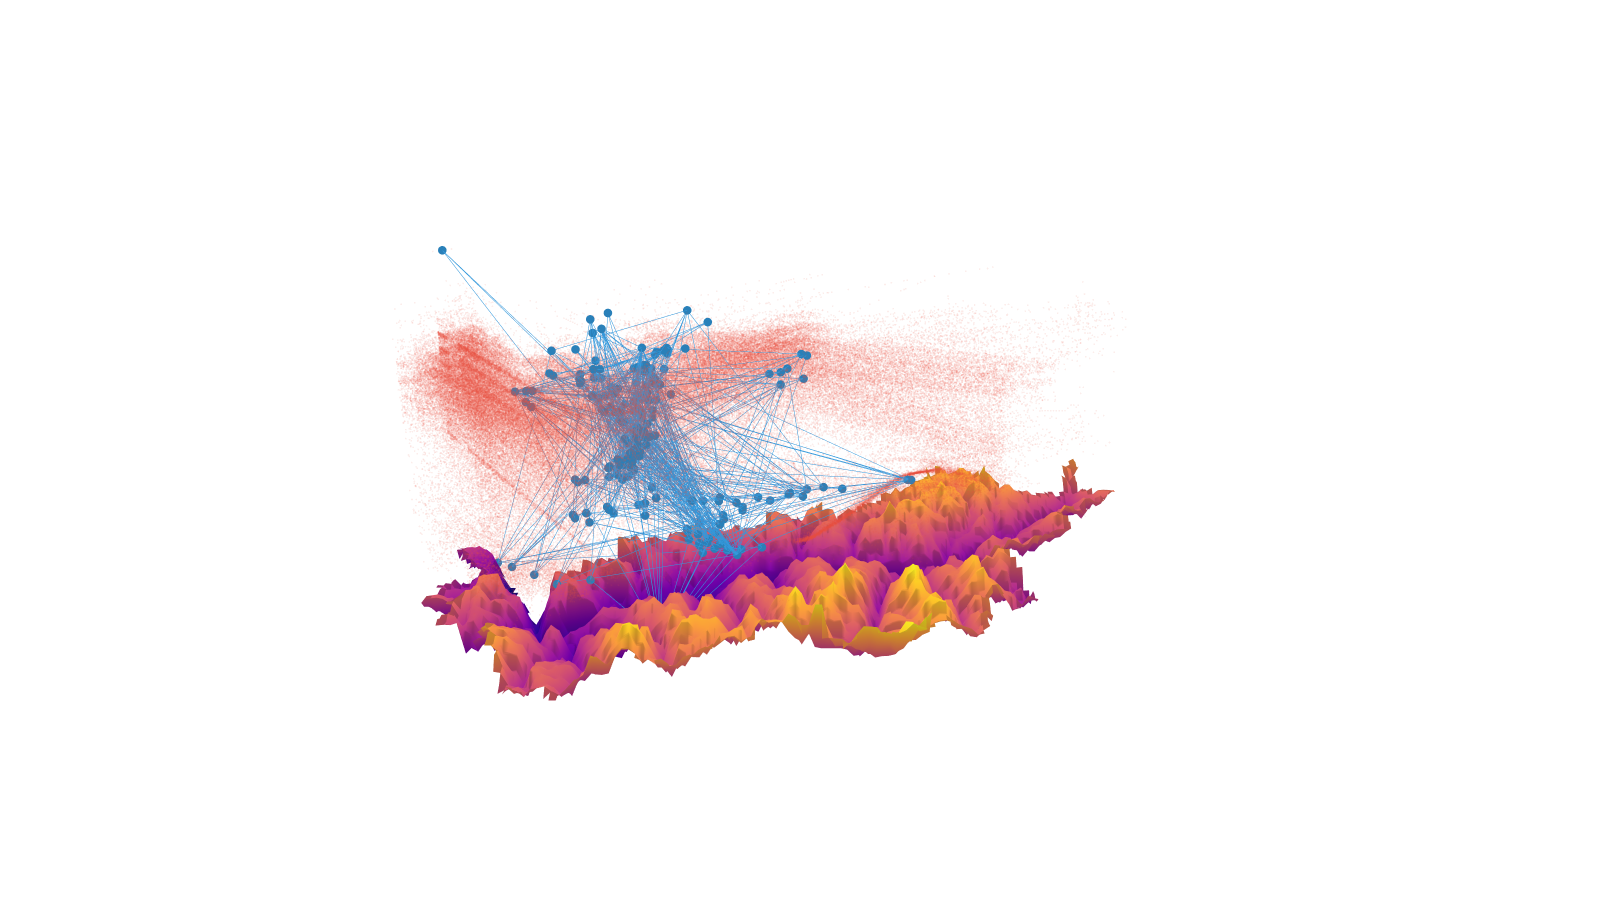
\includegraphics[trim={13cm 6cm 15cm 8cm},clip,width=\textwidth]{imgs/south-gen.png}
        \end{column}
    \end{columns}
\end{frame}

\begin{frame}
    \begin{columns}
        \begin{column}{0.5\textwidth}
            \begin{figure}[htbp]
                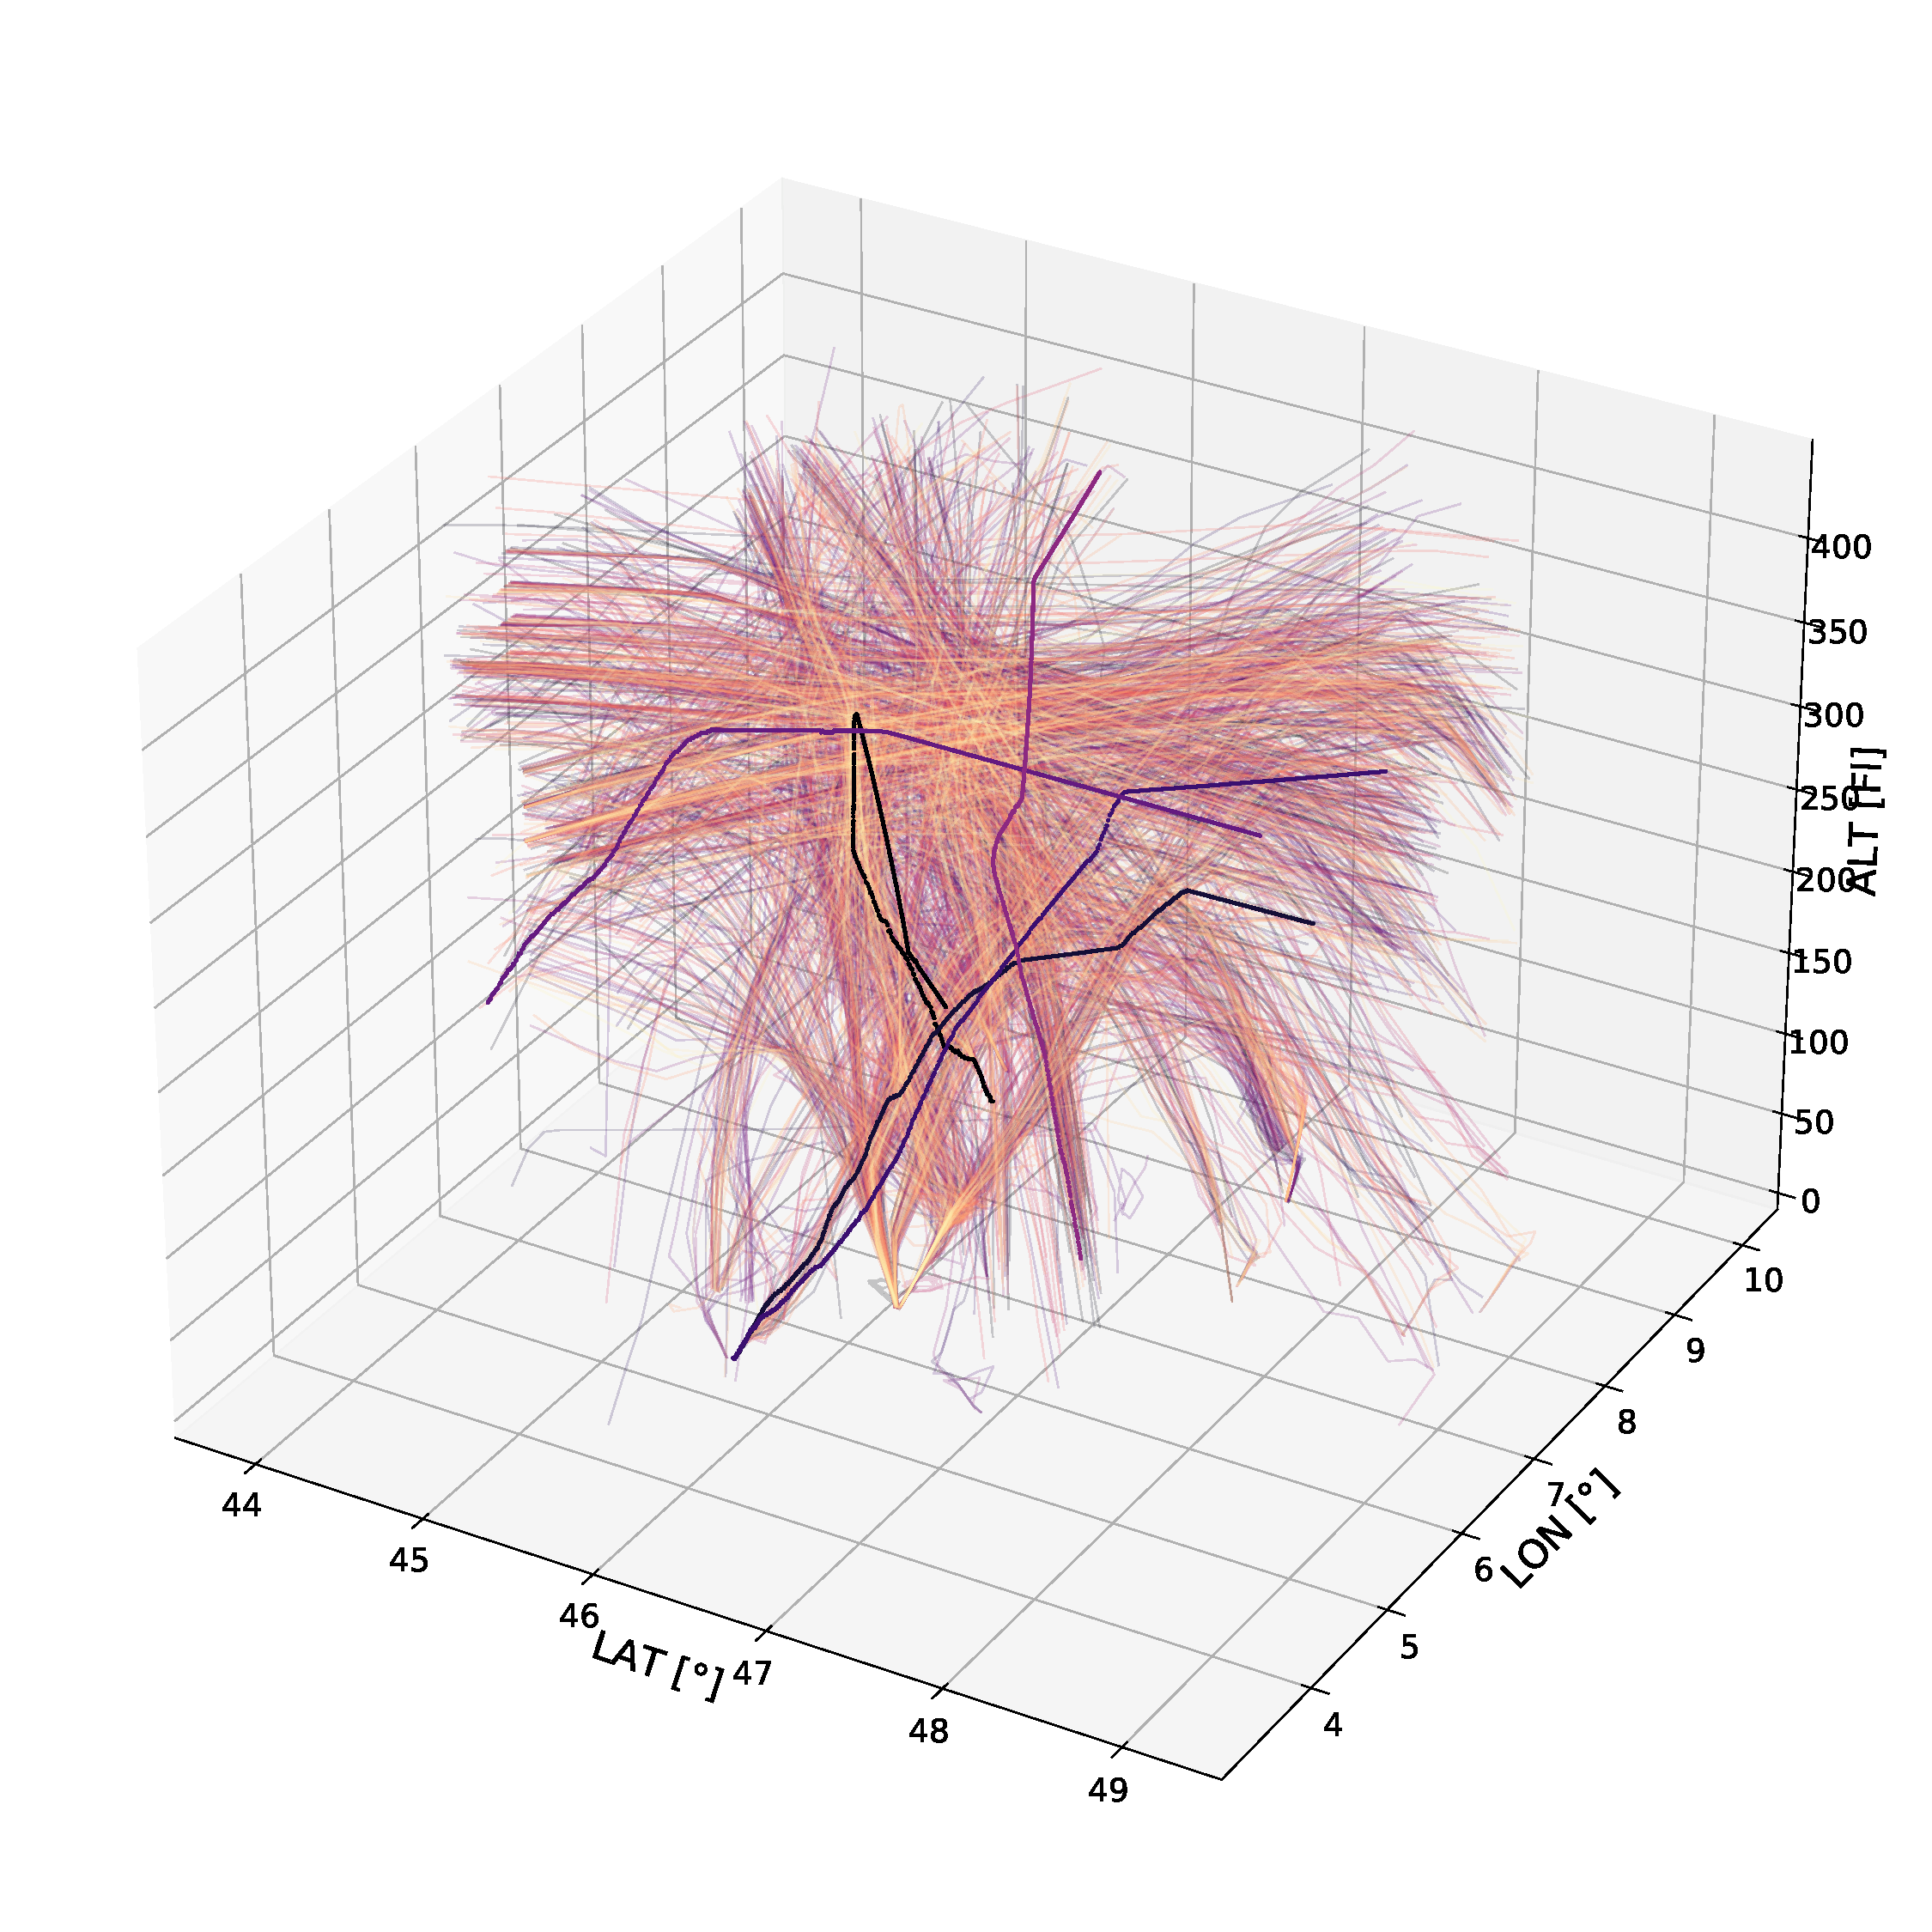
\includegraphics[height=0.83\textheight]{imgs/dataset.pdf}
            \end{figure}
        \end{column}
        \begin{column}{0.5\textwidth}
            \coltitle{SKYSOFT ATM MALAT Wind Speed Dataset}
            \vspace{10pt}
            \begin{itemize}
                \item Measures broadcasted every 4s
                \item Non-regular structure
                \item \url{https://www.idiap.ch/en/dataset/skysoft}
                \item \cite{skysoft2021dataset}
            \end{itemize}
            \begin{figure}[htbp]
                \centering
                \includegraphics[height=0.3\textheight]{beamer_theme/skysoft-logo.png}
            \end{figure}
        \end{column}
    \end{columns}
\end{frame}

\begin{frame}{\href{https://www.idiap.ch/en/dataset/skysoft}{SKYSOFT ATM MALAT Wind Speed Dataset}}
    \begin{columns}
        \begin{column}{0.5\textwidth}
            \begin{figure}[htbp]
                \centering
                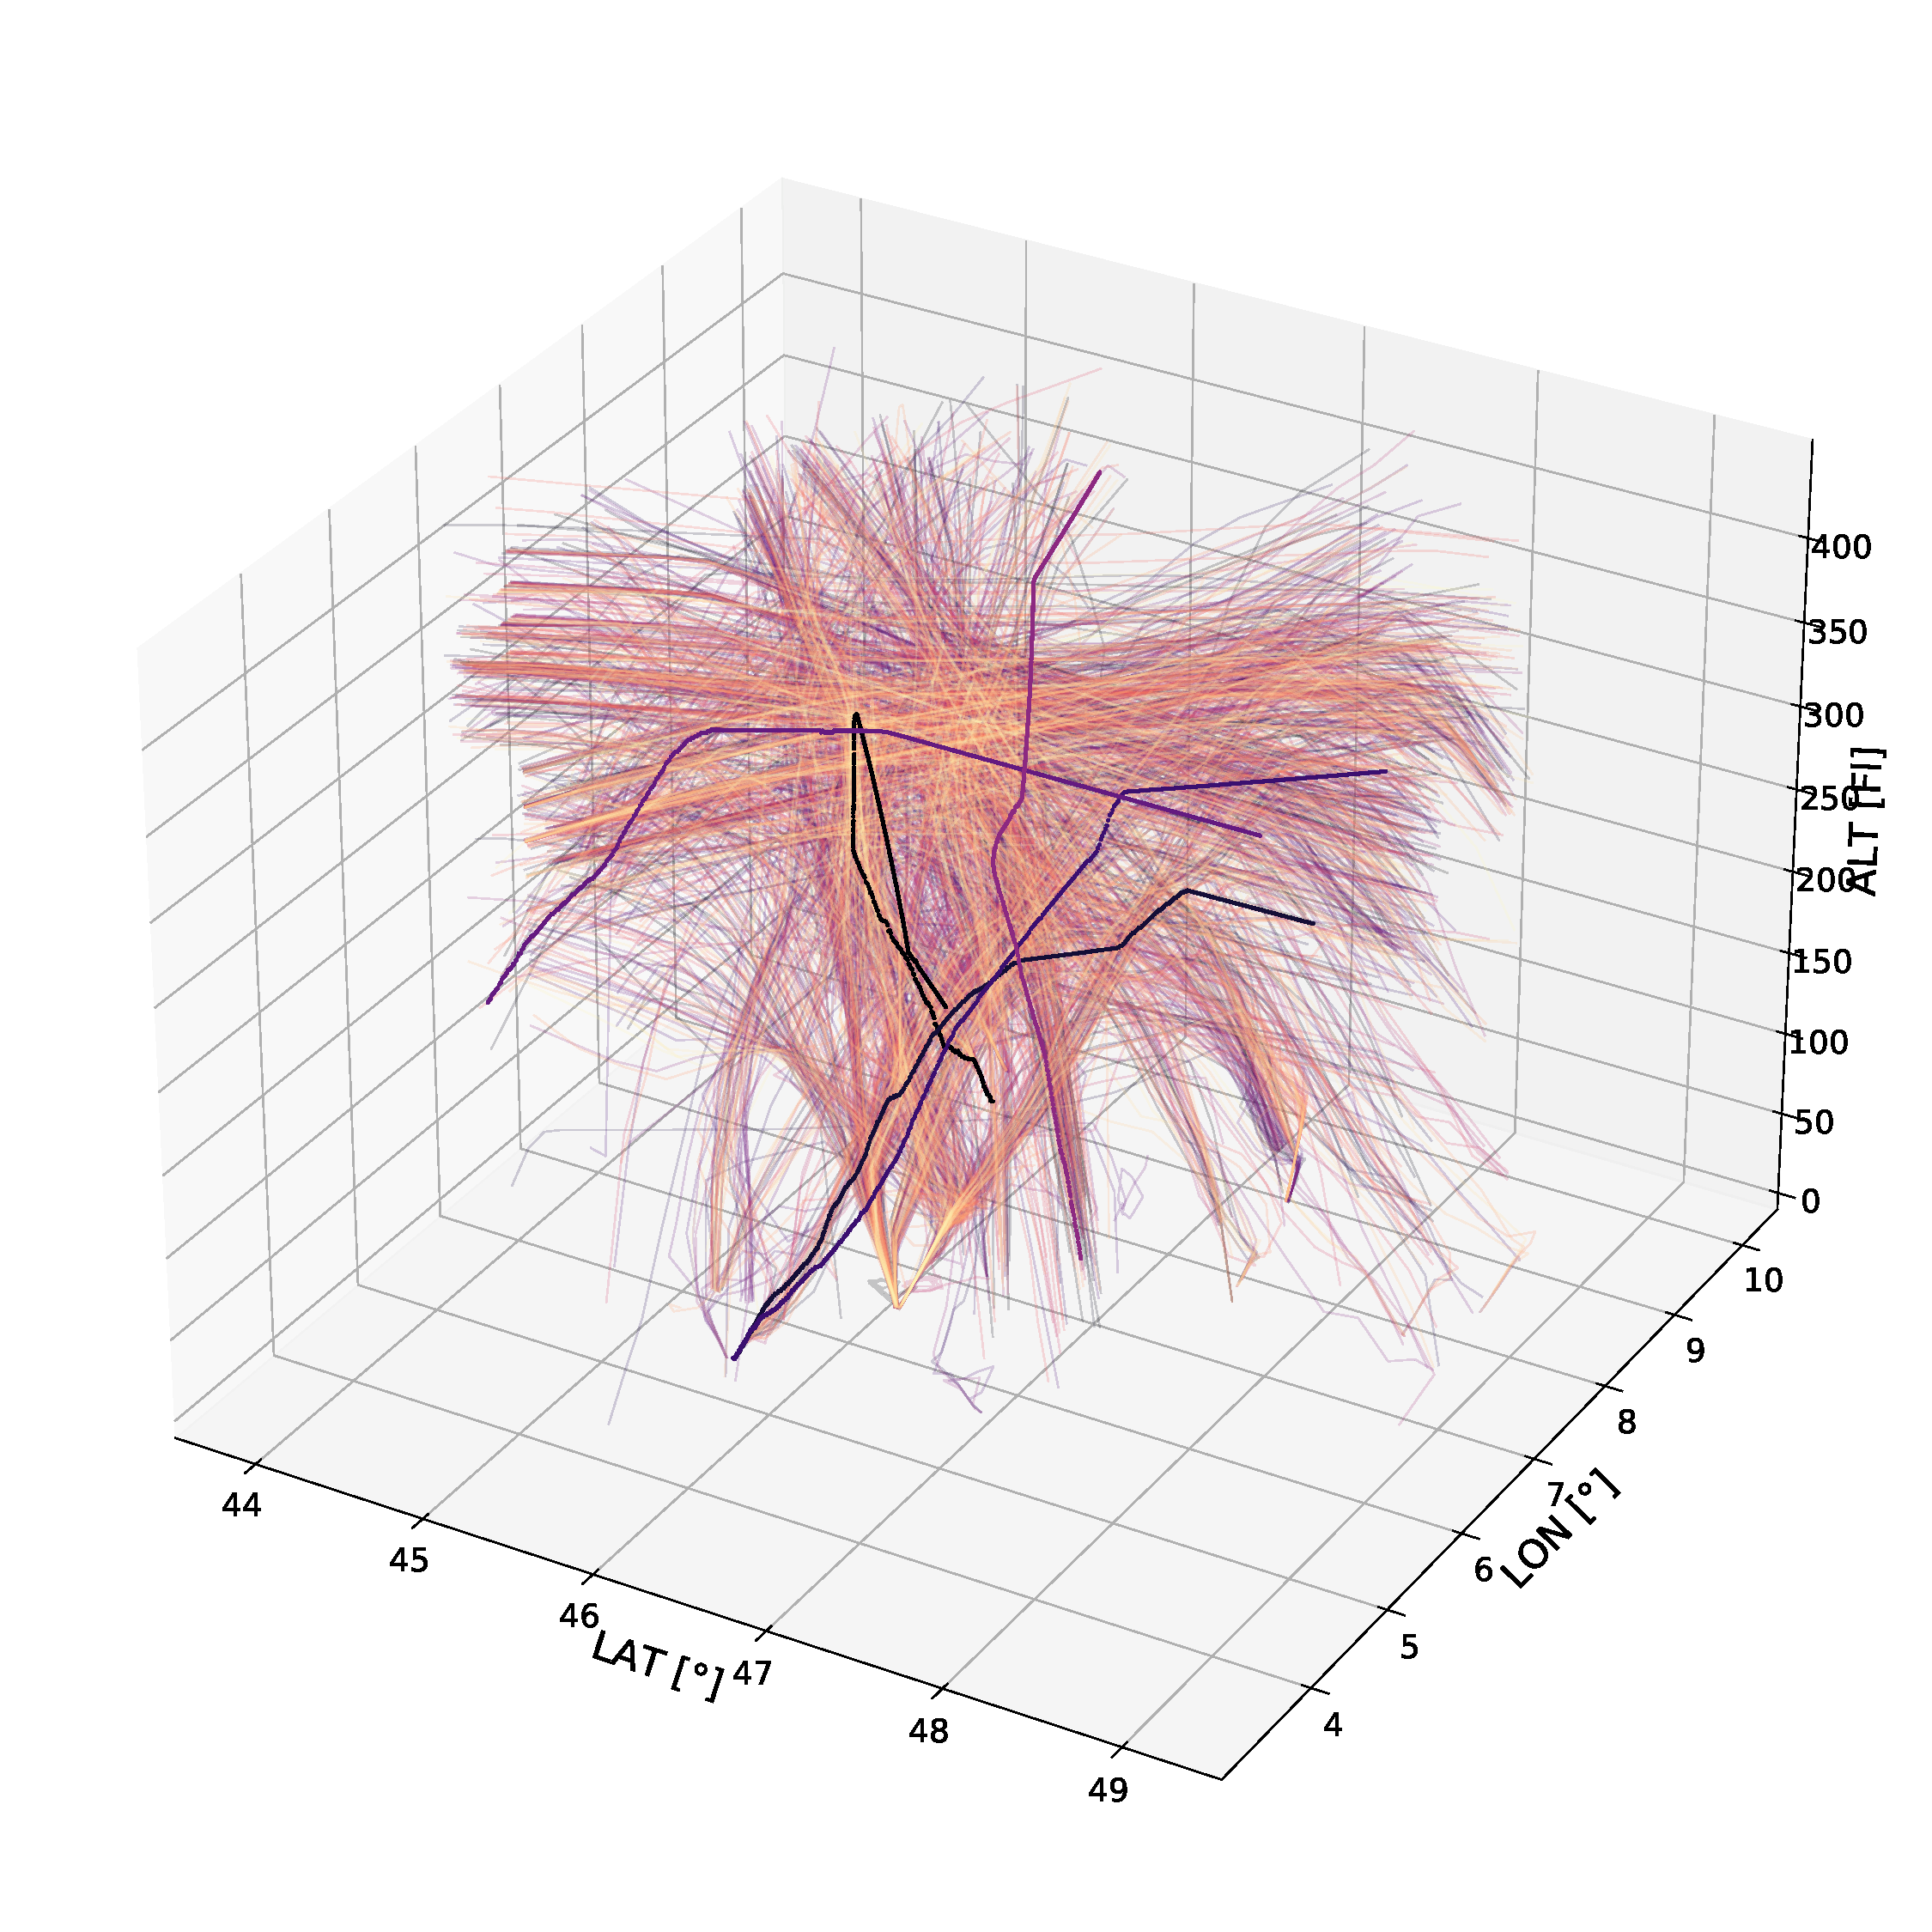
\includegraphics[height=0.6\textheight]{imgs/dataset.pdf}
                \caption{Measurements}
            \end{figure}
        \end{column}
        \begin{column}{0.5\textwidth}
            \begin{figure}[htbp]
                \centering
                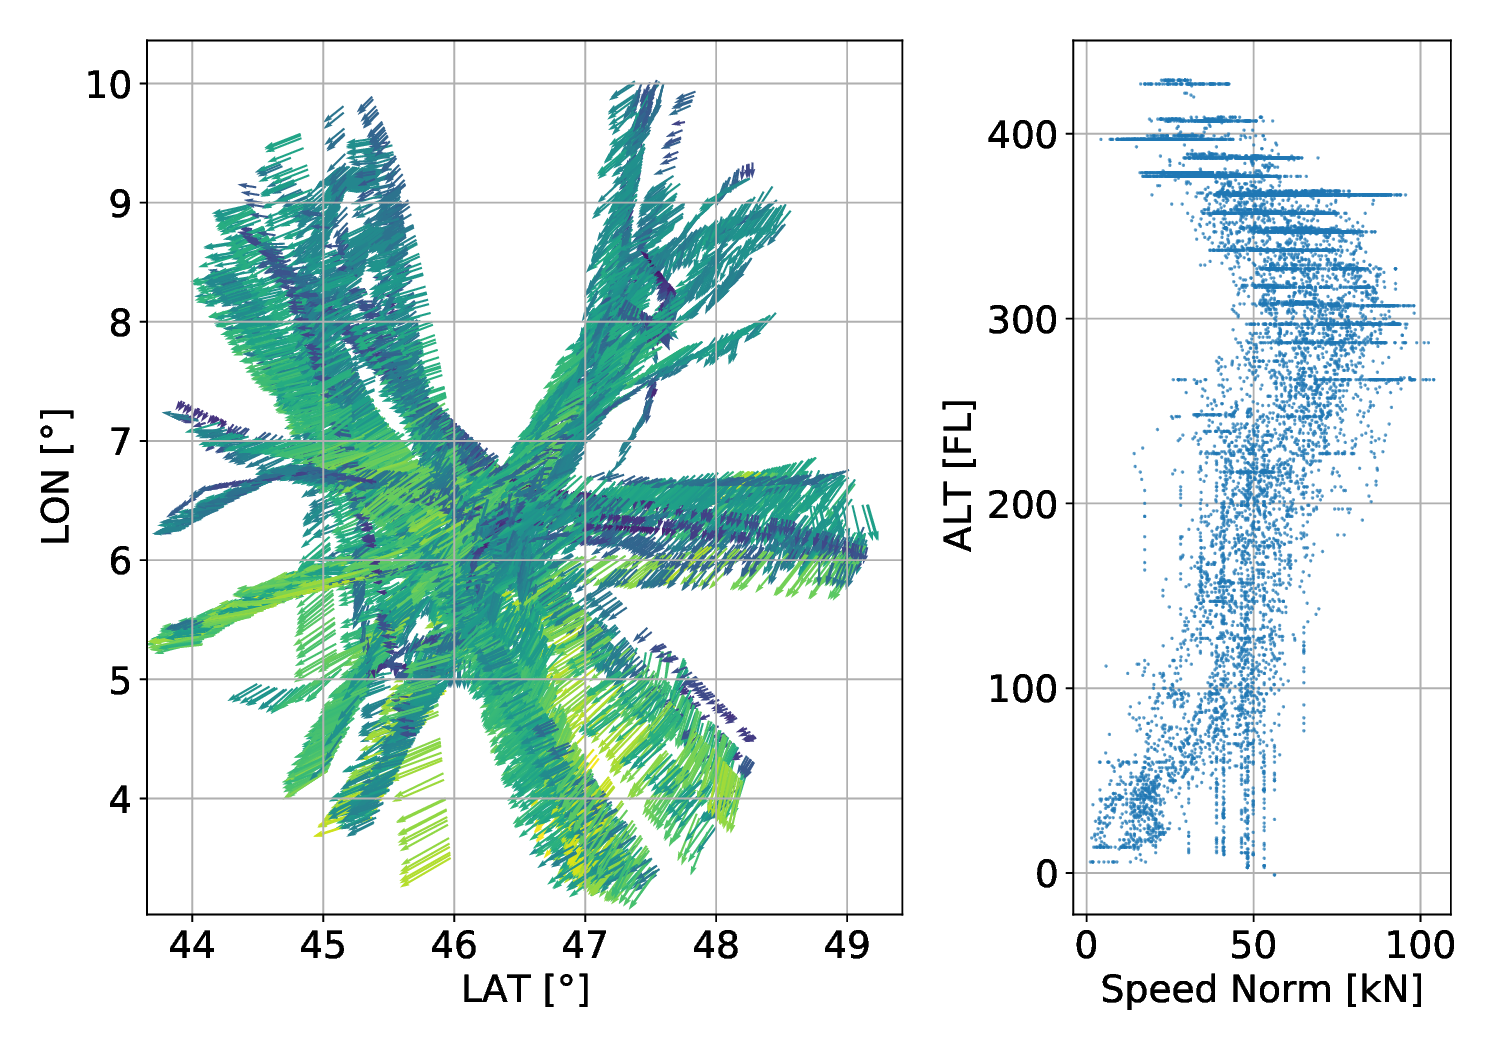
\includegraphics[height=0.5\textheight]{imgs/windspeed-rast.png}
                \caption{Wind Speed}
            \end{figure}
        \end{column}
    \end{columns}
\end{frame}

\begin{frame}{ Input $\rightarrow$ Target}
    \begin{columns}[T]
        \begin{column}{0.5\textwidth}
            \centering
            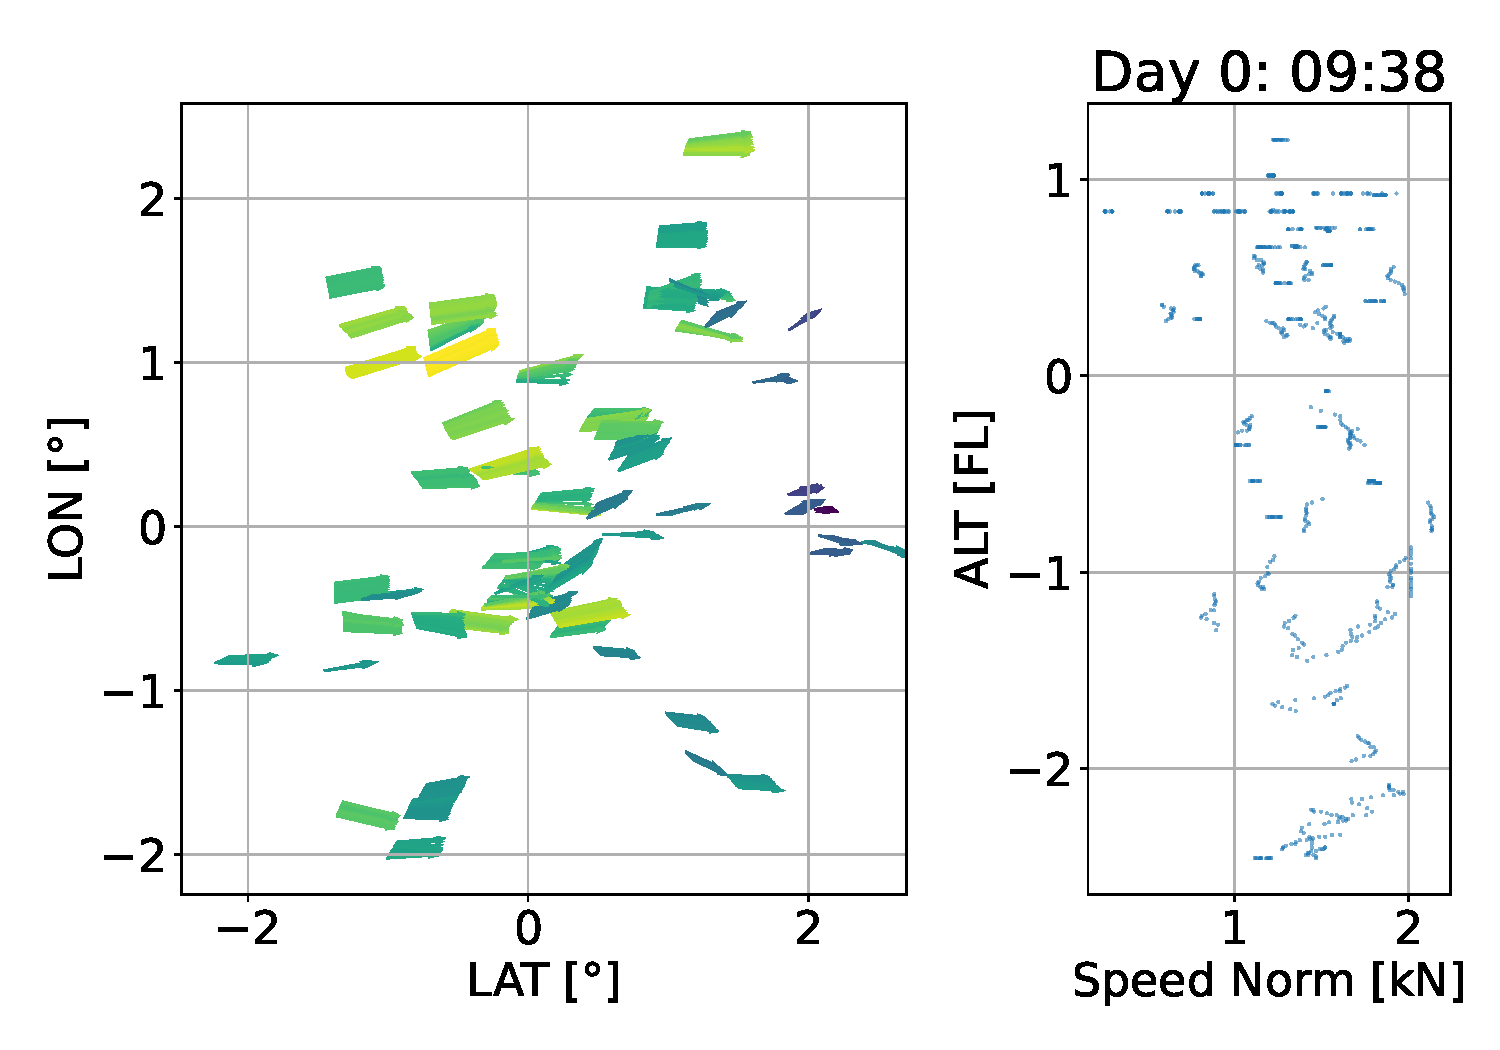
\includegraphics[height=0.6\textheight]{imgs/windslice-531}
        \end{column}
        \begin{column}{0.5\textwidth}
            \centering
            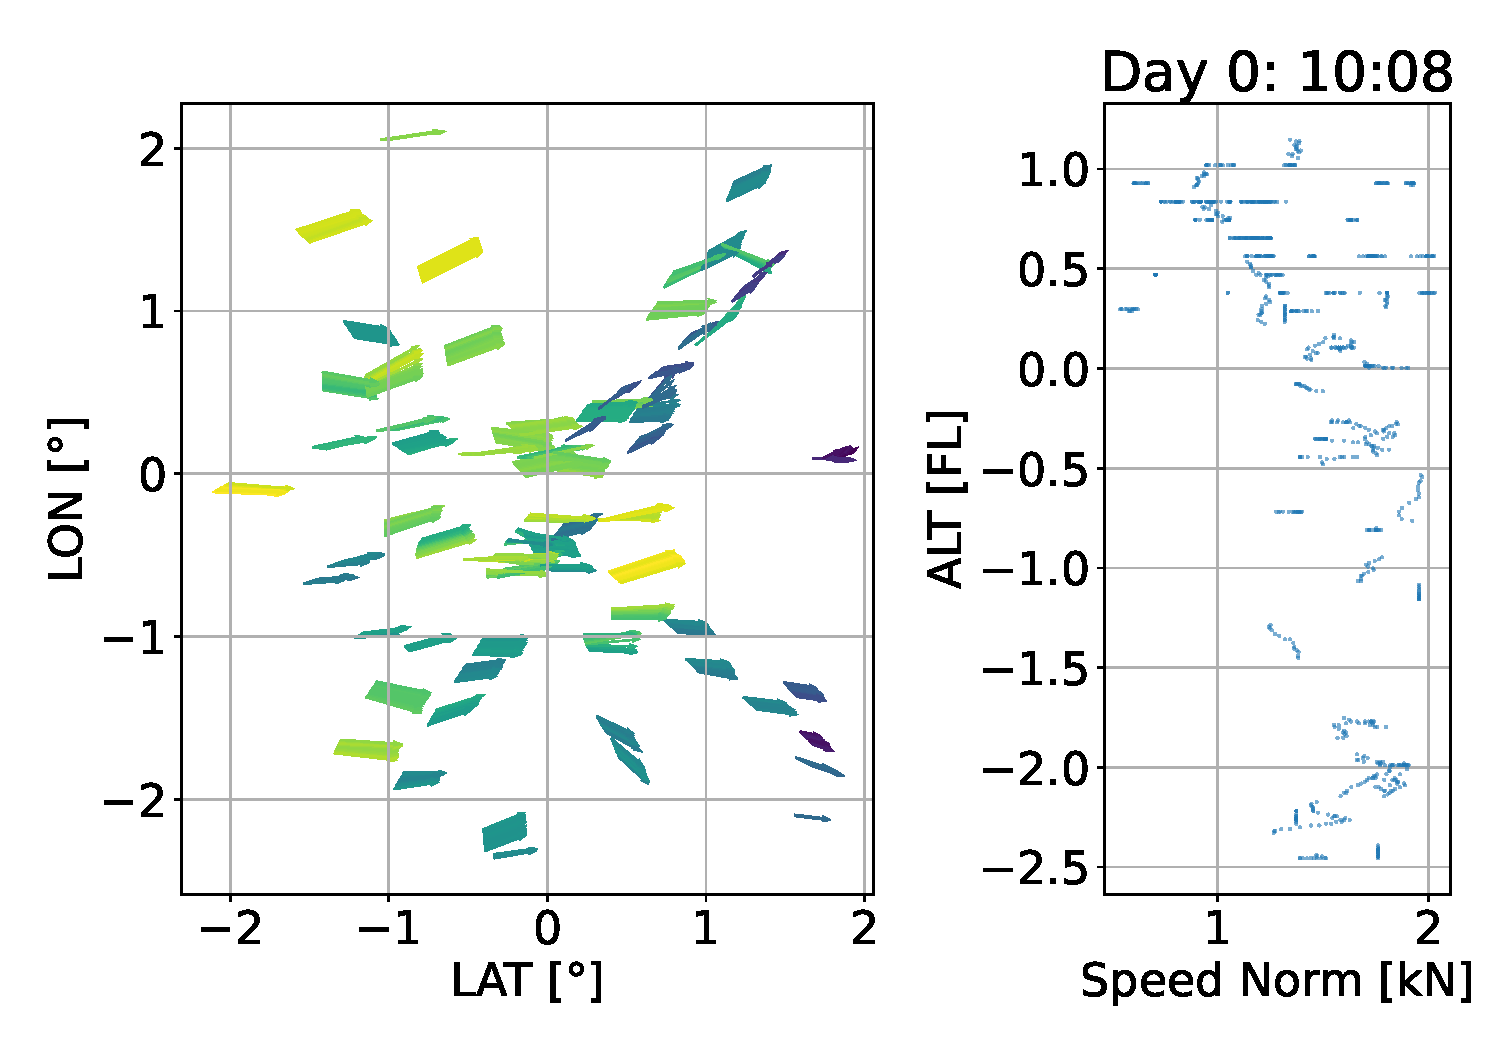
\includegraphics[height=0.6\textheight]{imgs/windslice-561}
        \end{column}
    \end{columns}
\end{frame}

\begin{frame}
    \begin{columns}
        \begin{column}{0.5\textwidth}
            \centering
            \begin{tcolorbox}[height=2.8in, width=2.2in, enhanced, fuzzy shadow={0mm}{-1pt}{-0.5pt}{0.4mm}{black!80!white}, boxrule=0.4pt,sharp corners,colframe=black,colback=white]
                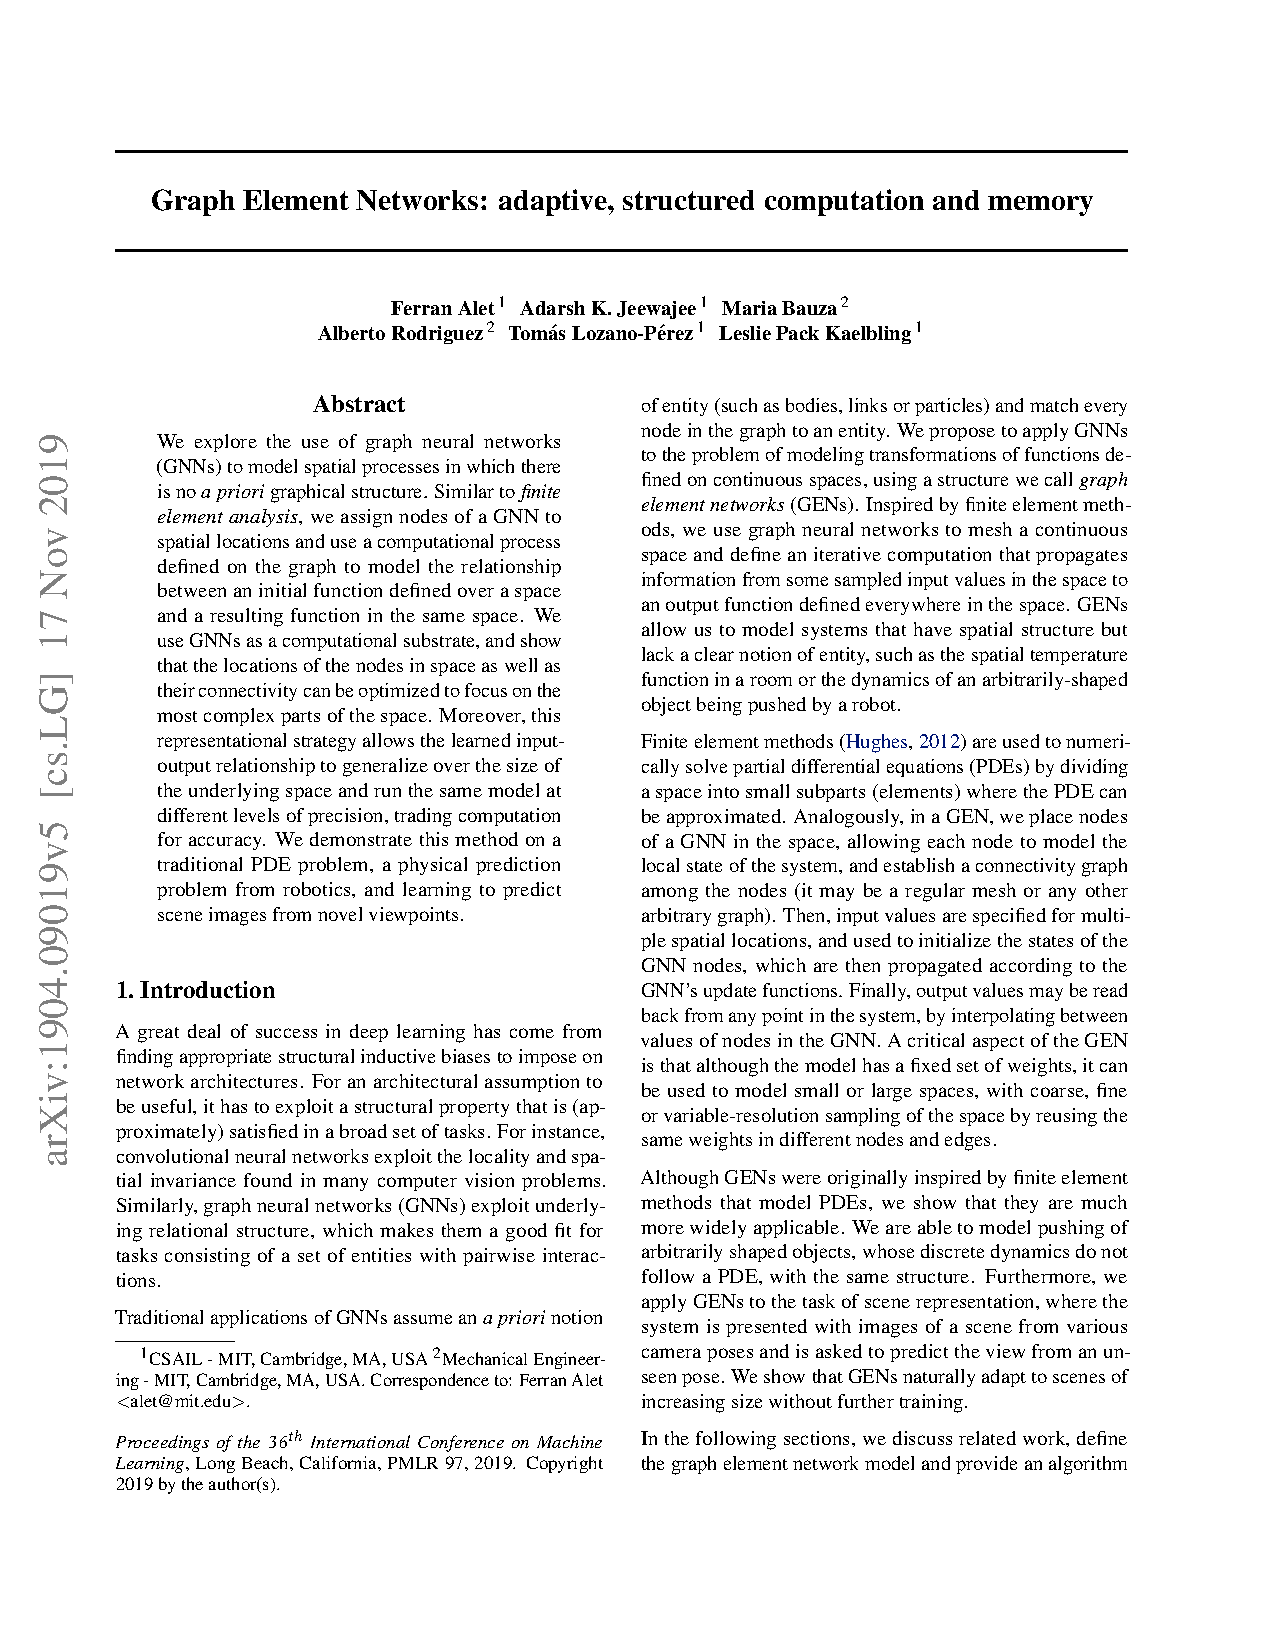
\includegraphics[height=2.4in]{imgs/gen-1p}
            \end{tcolorbox}
        \end{column}
        \begin{column}{0.5\textwidth}
            \huge \bfseries \color{black}
            Graph Element Networks \cite{alet2019graph}
        \end{column}
    \end{columns}
\end{frame}


\begin{frame}{GEN Architecture}
    \begin{figure}[htbp]
        \centering
        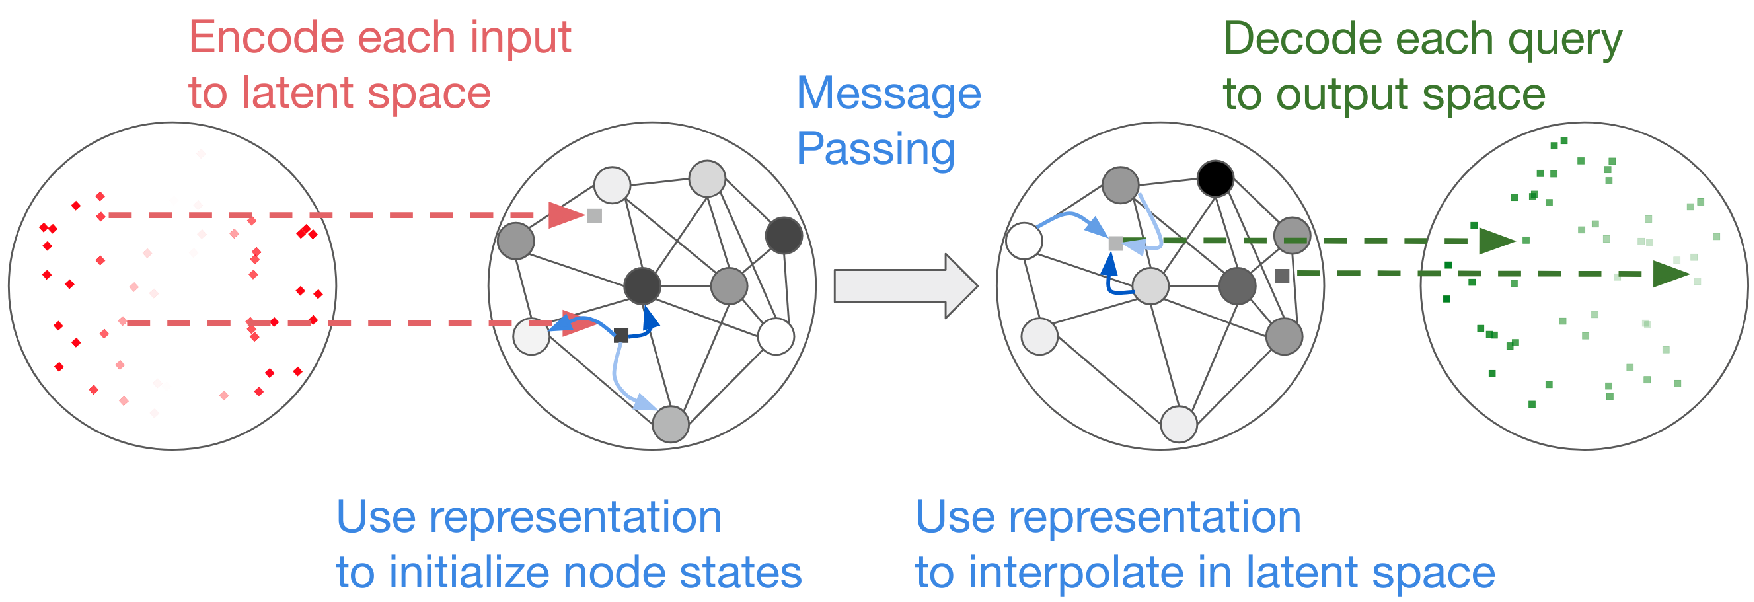
\includegraphics[width=\textwidth]{imgs/gen-fig}
    \end{figure}
\end{frame}
\begin{frame}[plain]{Graph Types}
    \begin{figure}[htbp]
        \begin{subfigure}{0.24\textwidth}
            \centering
            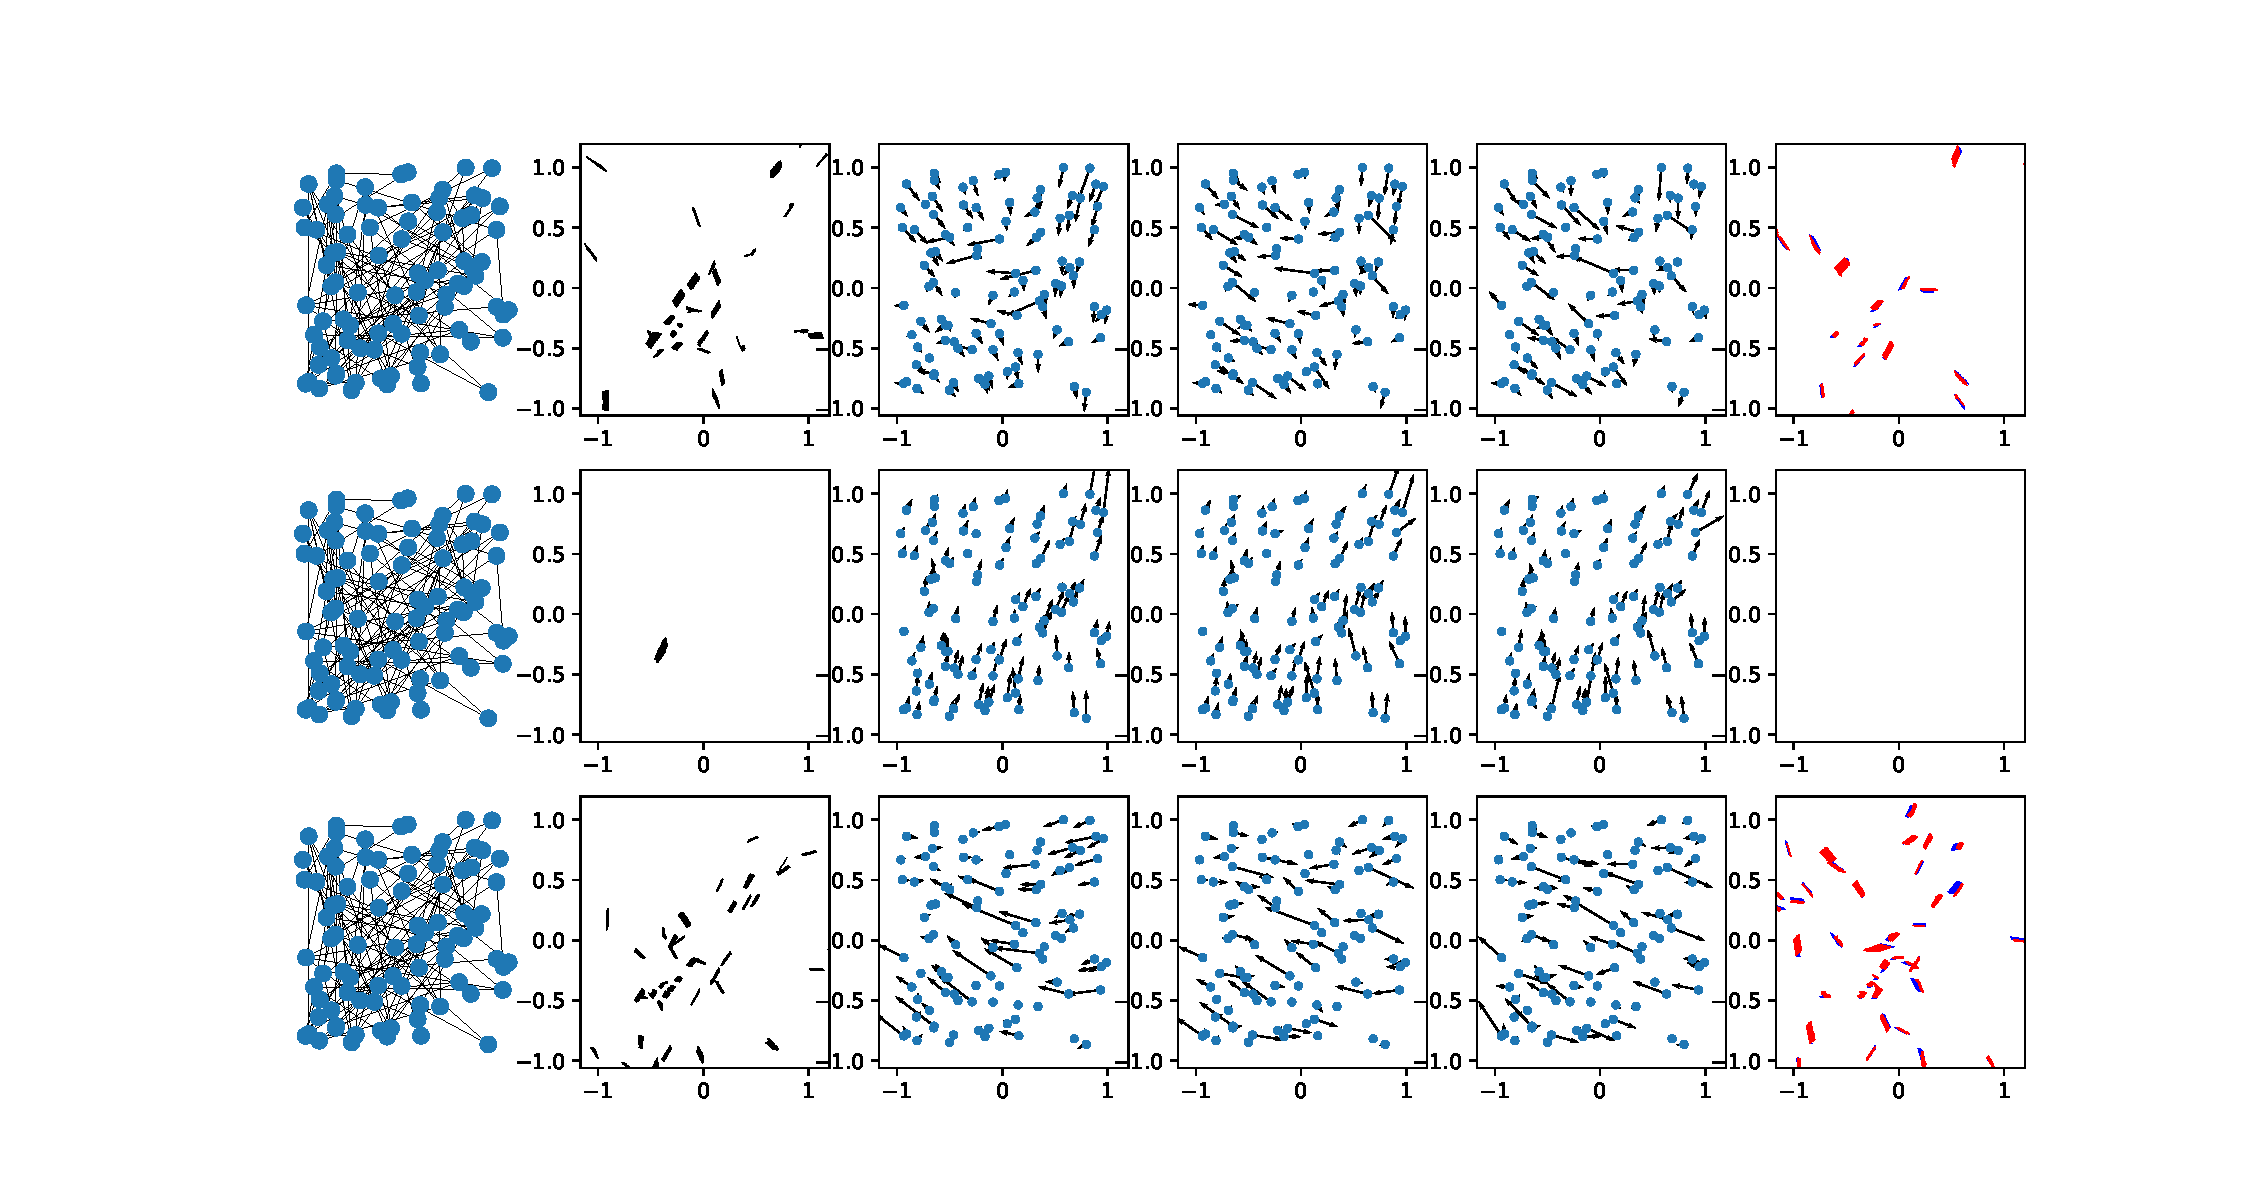
\includegraphics[trim={4.8cm 13.2cm 29.3cm 2.4cm},clip,width=0.7\textwidth]{../results/pdfs/rn1-100N-noemb-fixed}
            \caption{Random network with $p=1\%$}
        \end{subfigure}
        \begin{subfigure}{0.24\textwidth}
            \centering
            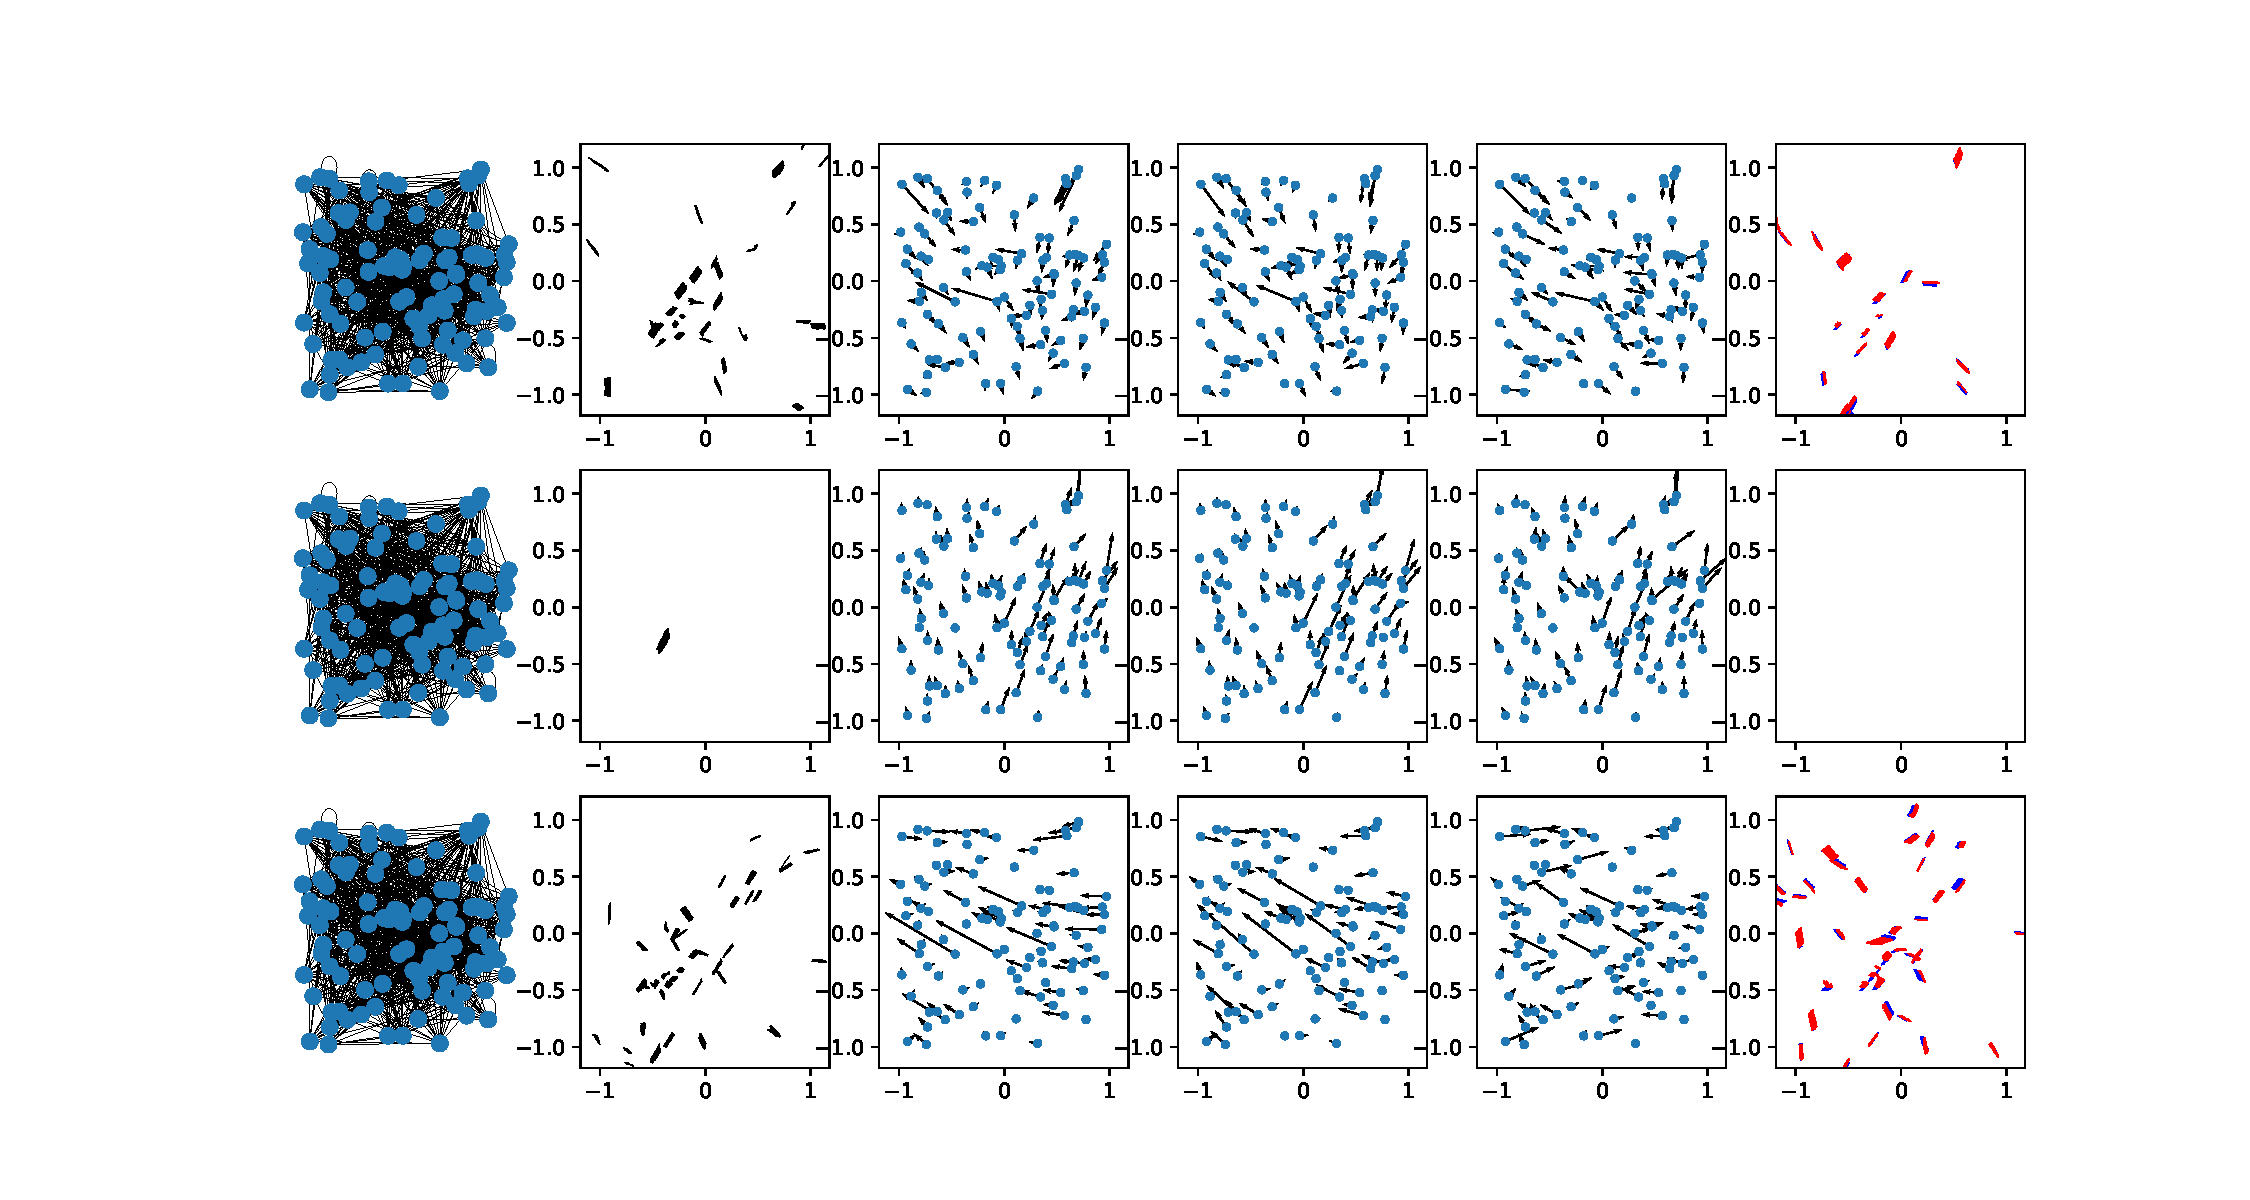
\includegraphics[trim={4.8cm 13.2cm 29.3cm 2.4cm},clip,width=0.7\textwidth]{../results/pdfs/rn10-100N-noemb-fixed}
            \caption{Random network with $p=10\%$}
        \end{subfigure}
        \begin{subfigure}{0.24\textwidth}
            \centering
            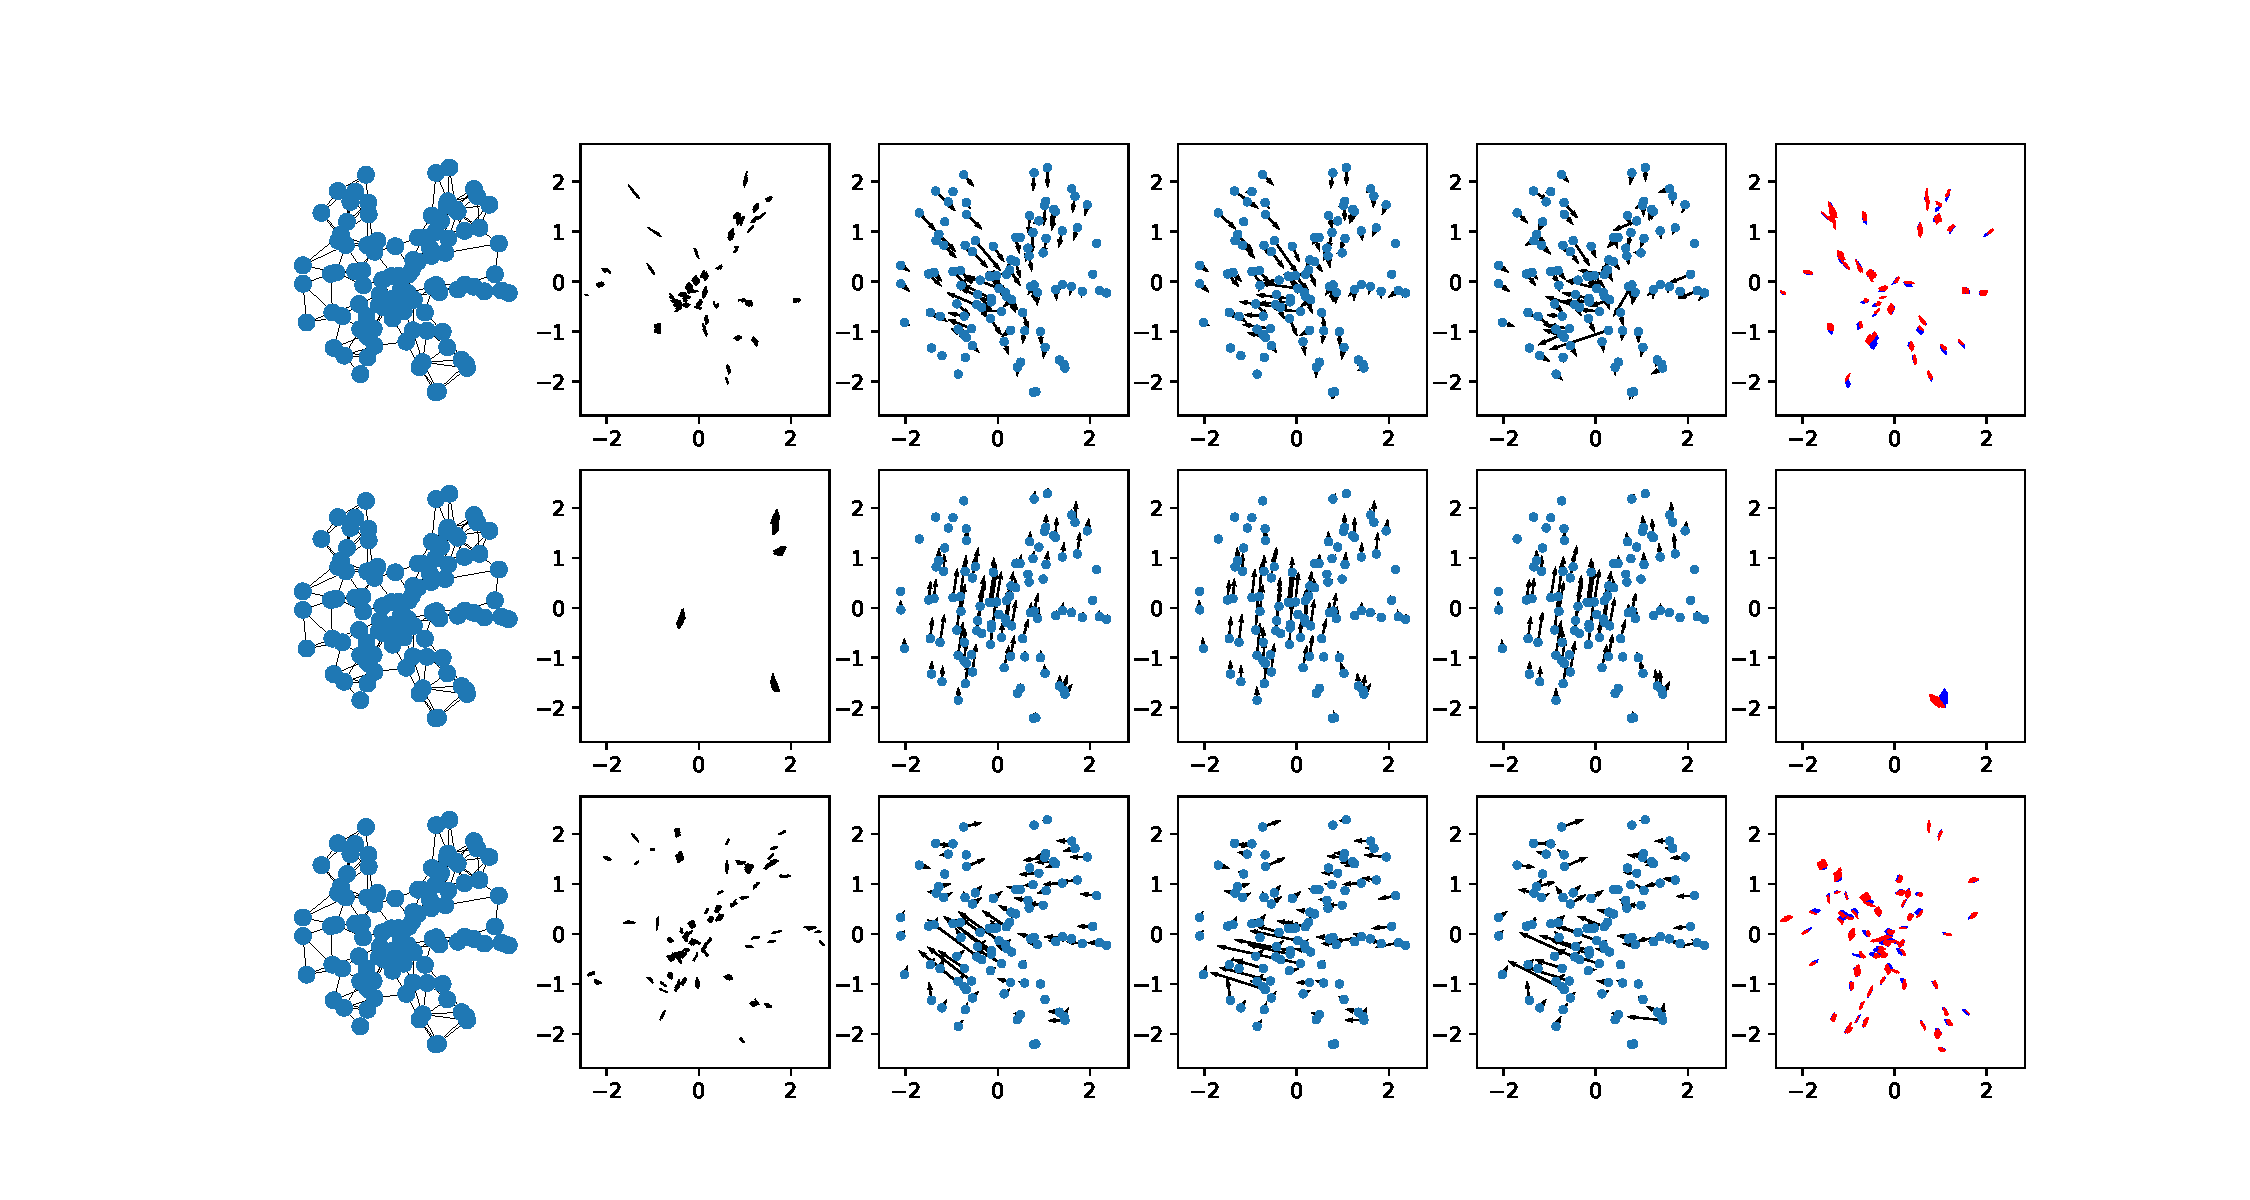
\includegraphics[trim={4.8cm 13.2cm 29.3cm 2.4cm},clip,width=0.7\textwidth]{../results/pdfs/nn-100N-noemb-fixed}
            \caption{$k$-means, 3nn}
        \end{subfigure}
        \begin{subfigure}{0.24\textwidth}
            \centering
            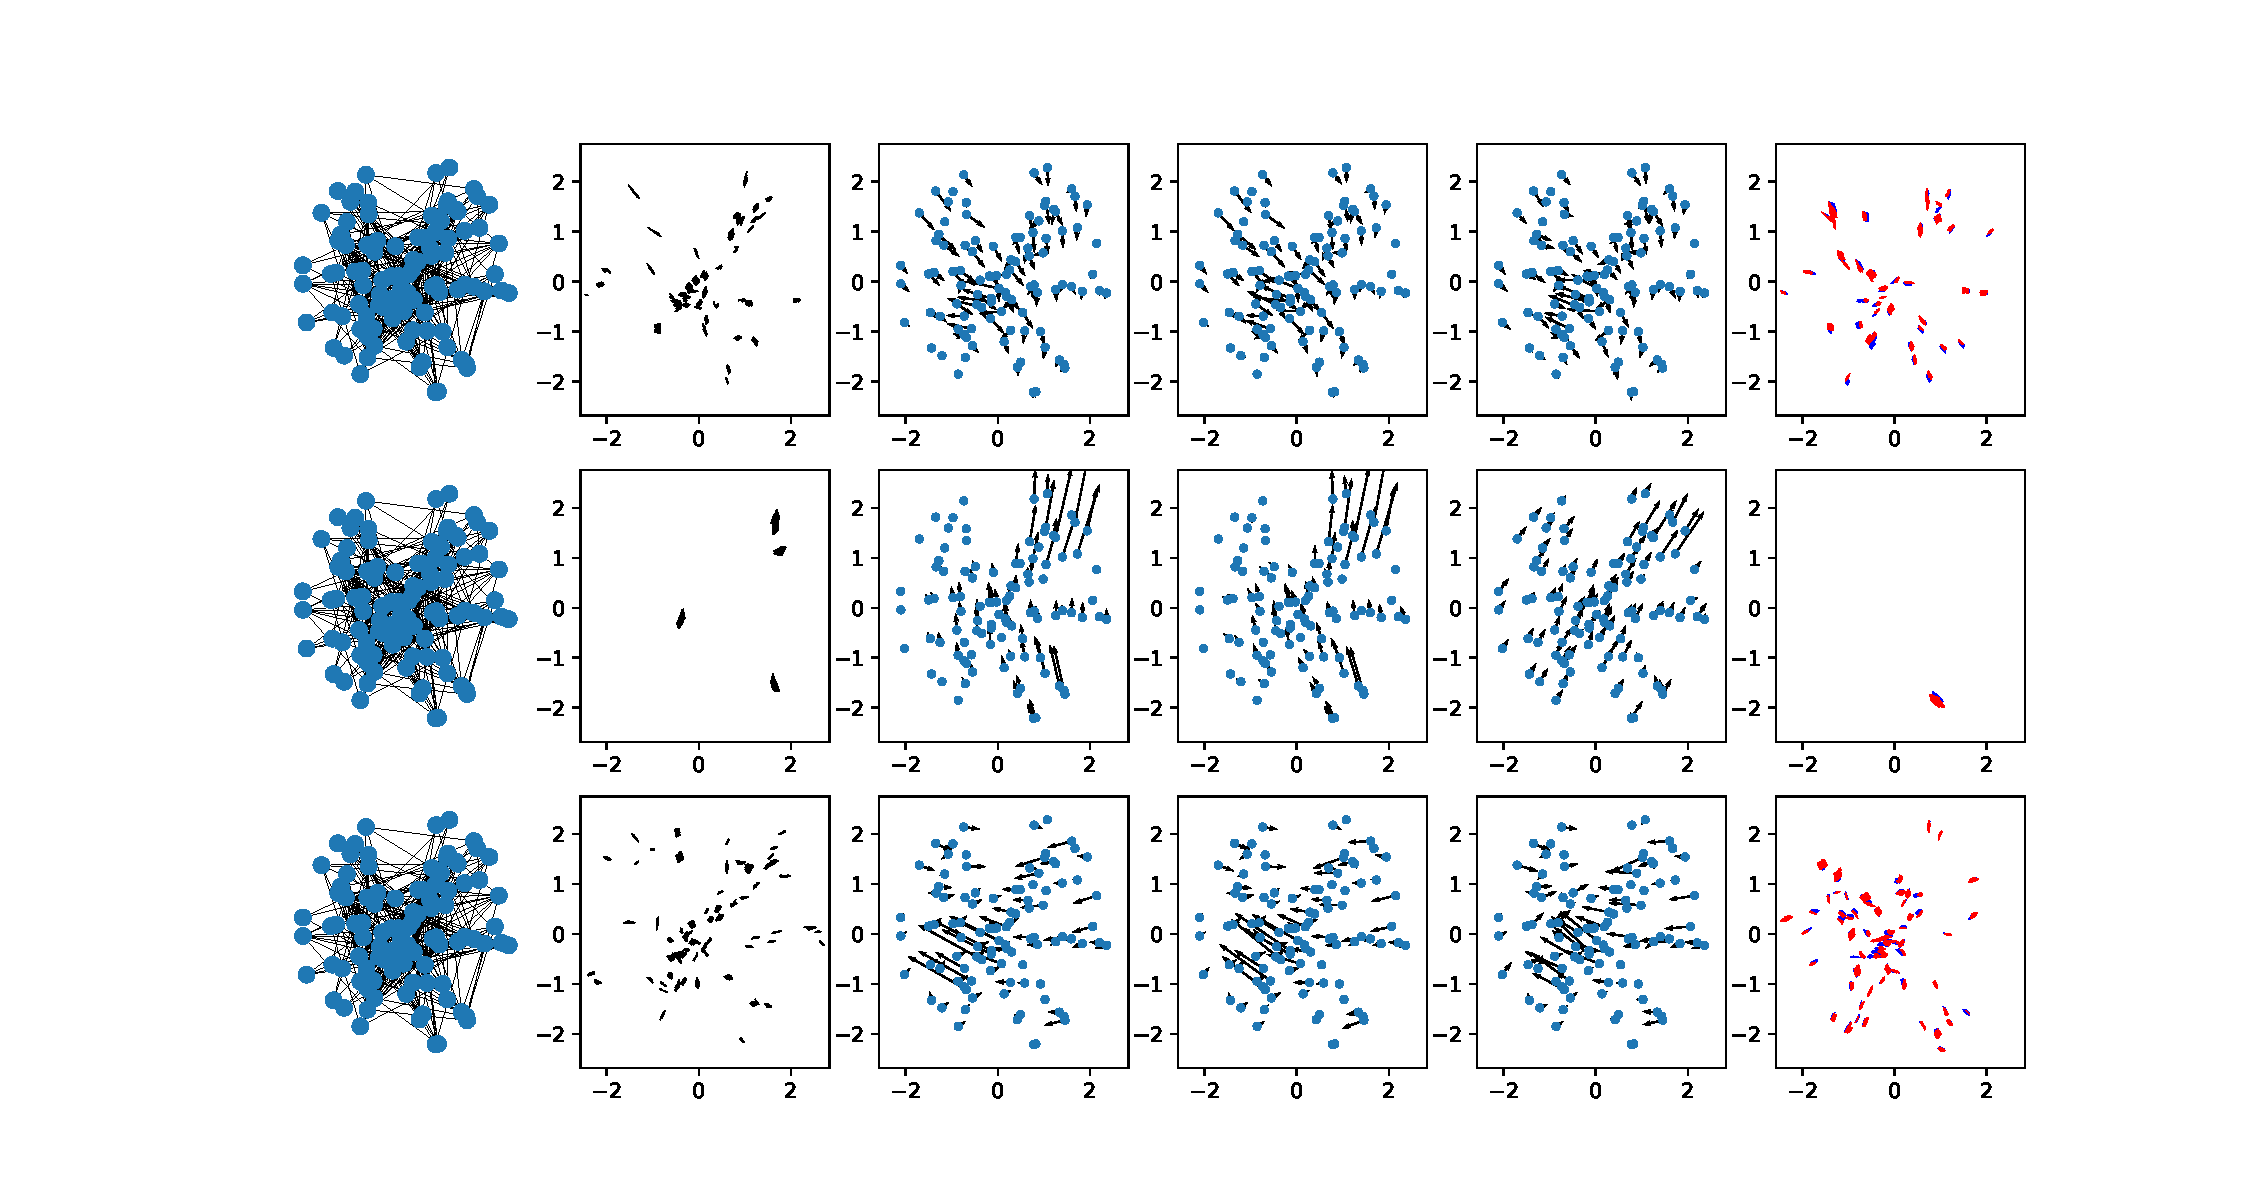
\includegraphics[trim={4.8cm 13.2cm 29.3cm 2.4cm},clip,width=0.7\textwidth]{../results/pdfs/ba-100N-noemb-fixed}
            \caption{$k$-means, BA}
        \end{subfigure}
        \pause
        \begin{subfigure}{0.24\textwidth}
            \centering
            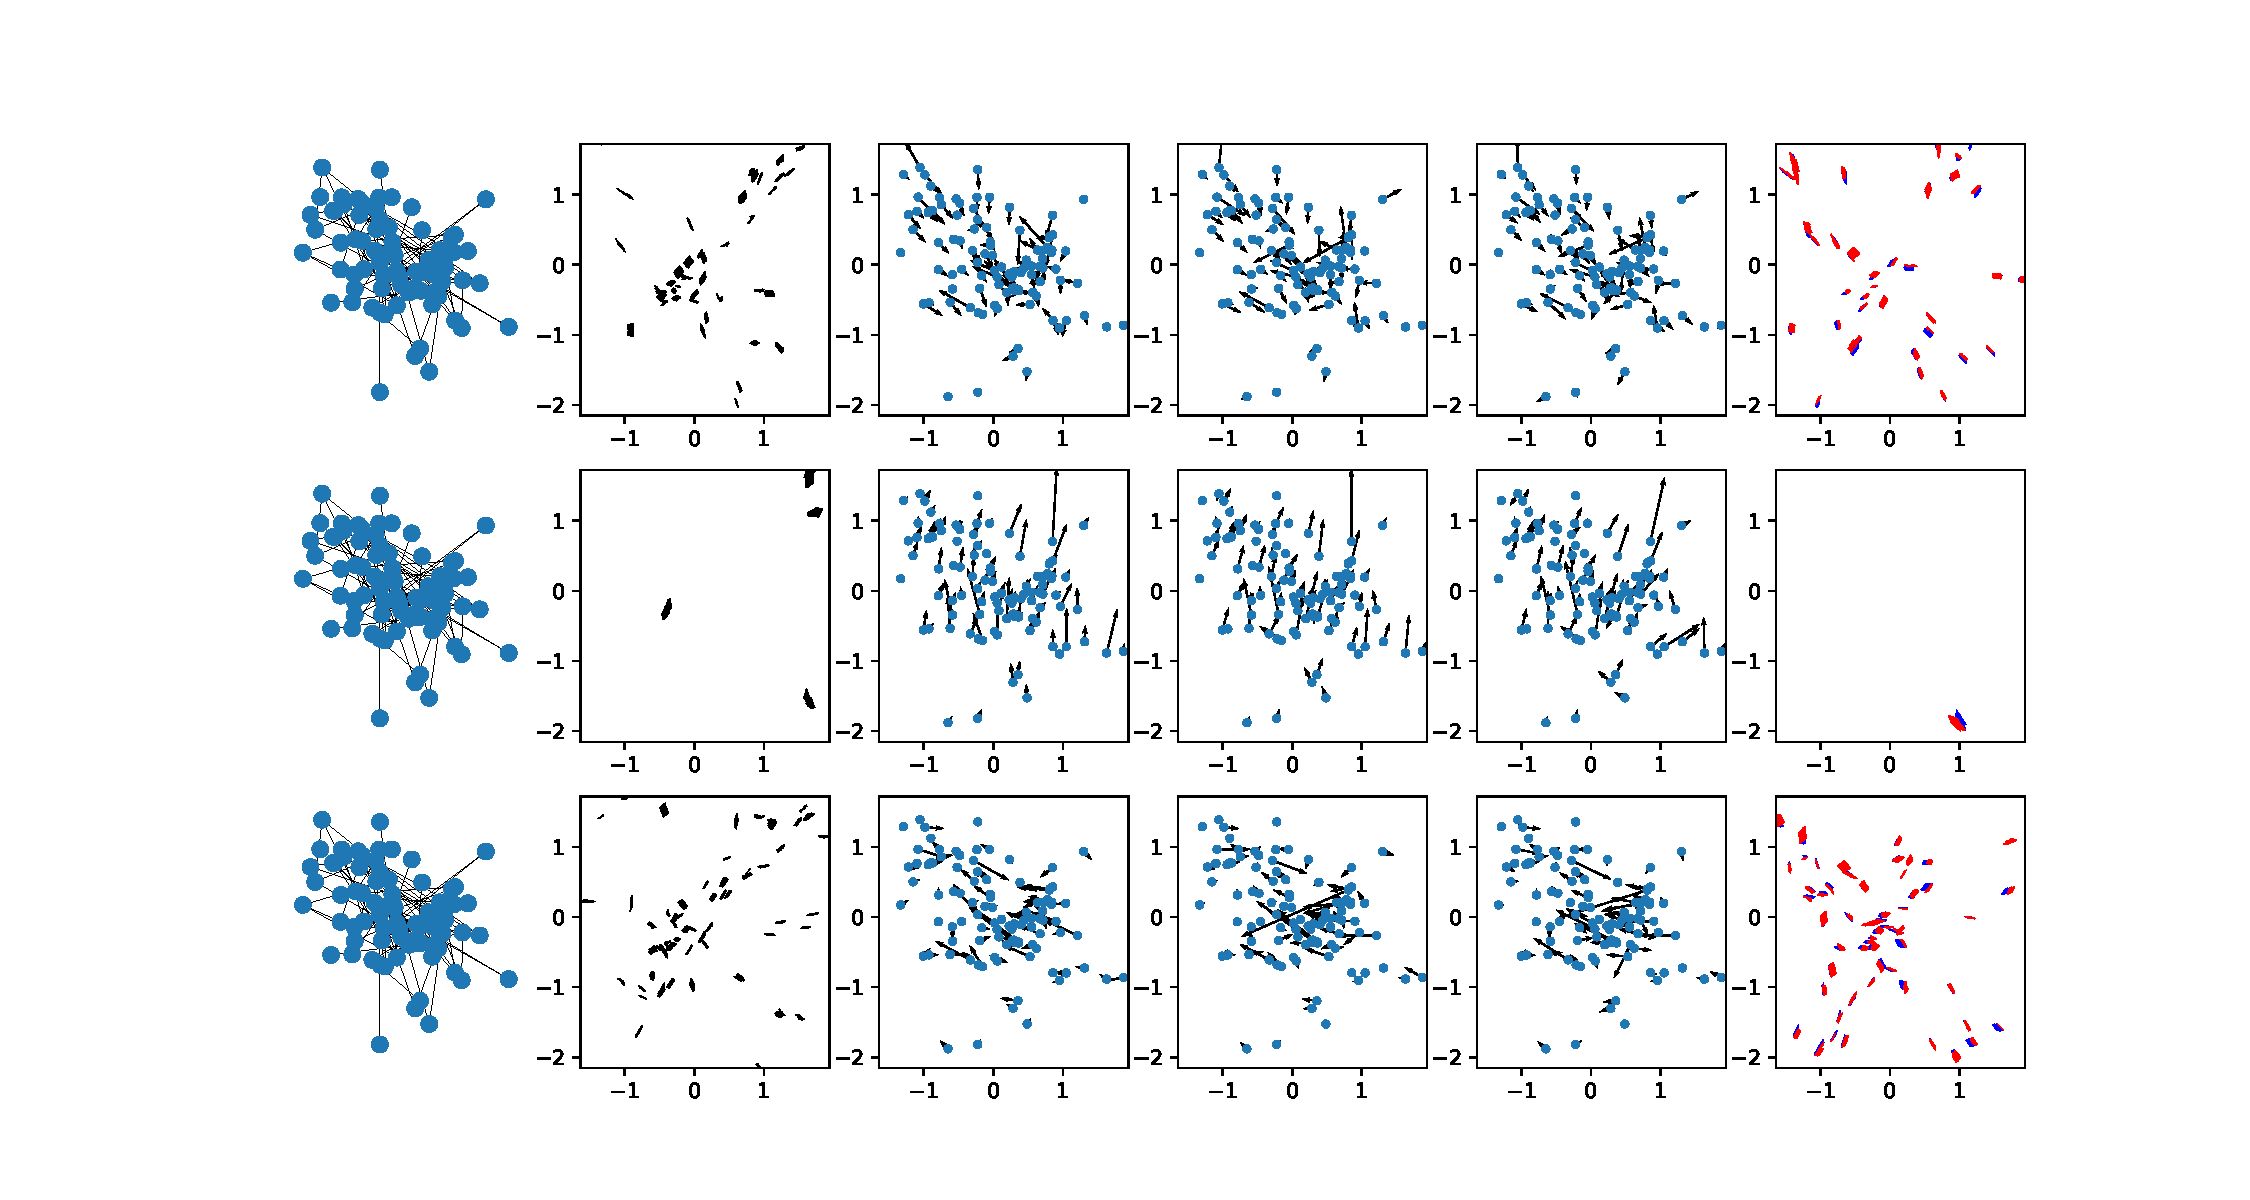
\includegraphics[trim={4.8cm 13.2cm 29.3cm 2.4cm},clip,width=0.7\textwidth]{../results/pdfs/rn1-100N-noemb0}
            \caption{Random network with $p=1\%$}
        \end{subfigure}
        \begin{subfigure}{0.24\textwidth}
            \centering
            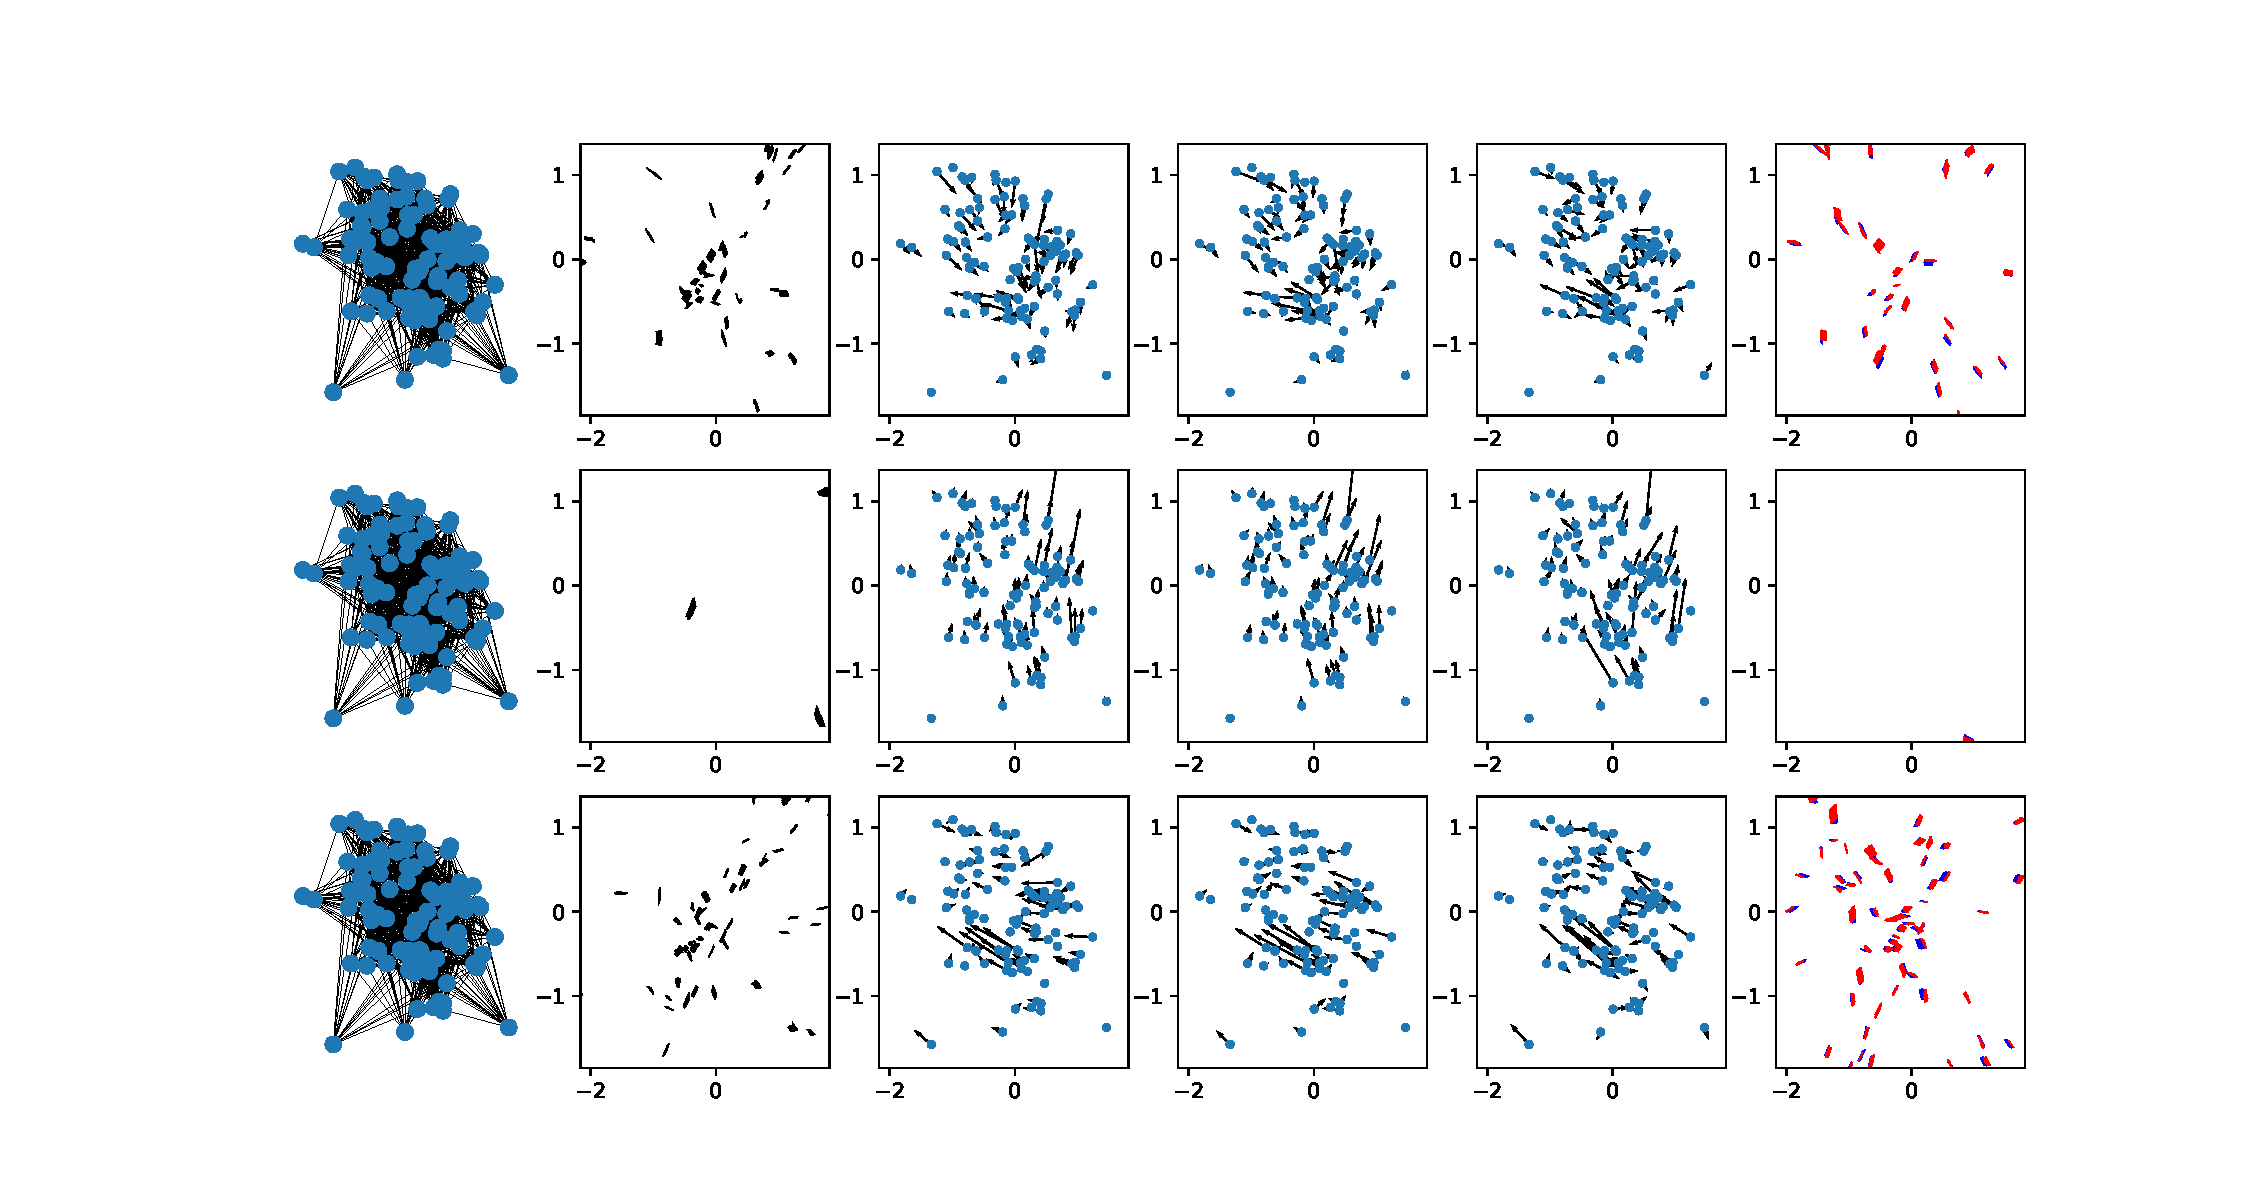
\includegraphics[trim={4.8cm 13.2cm 29.3cm 2.4cm},clip,width=0.7\textwidth]{../results/pdfs/rn10-100N-noemb0}
            \caption{Random network with $p=10\%$}
        \end{subfigure}
        \begin{subfigure}{0.24\textwidth}
            \centering
            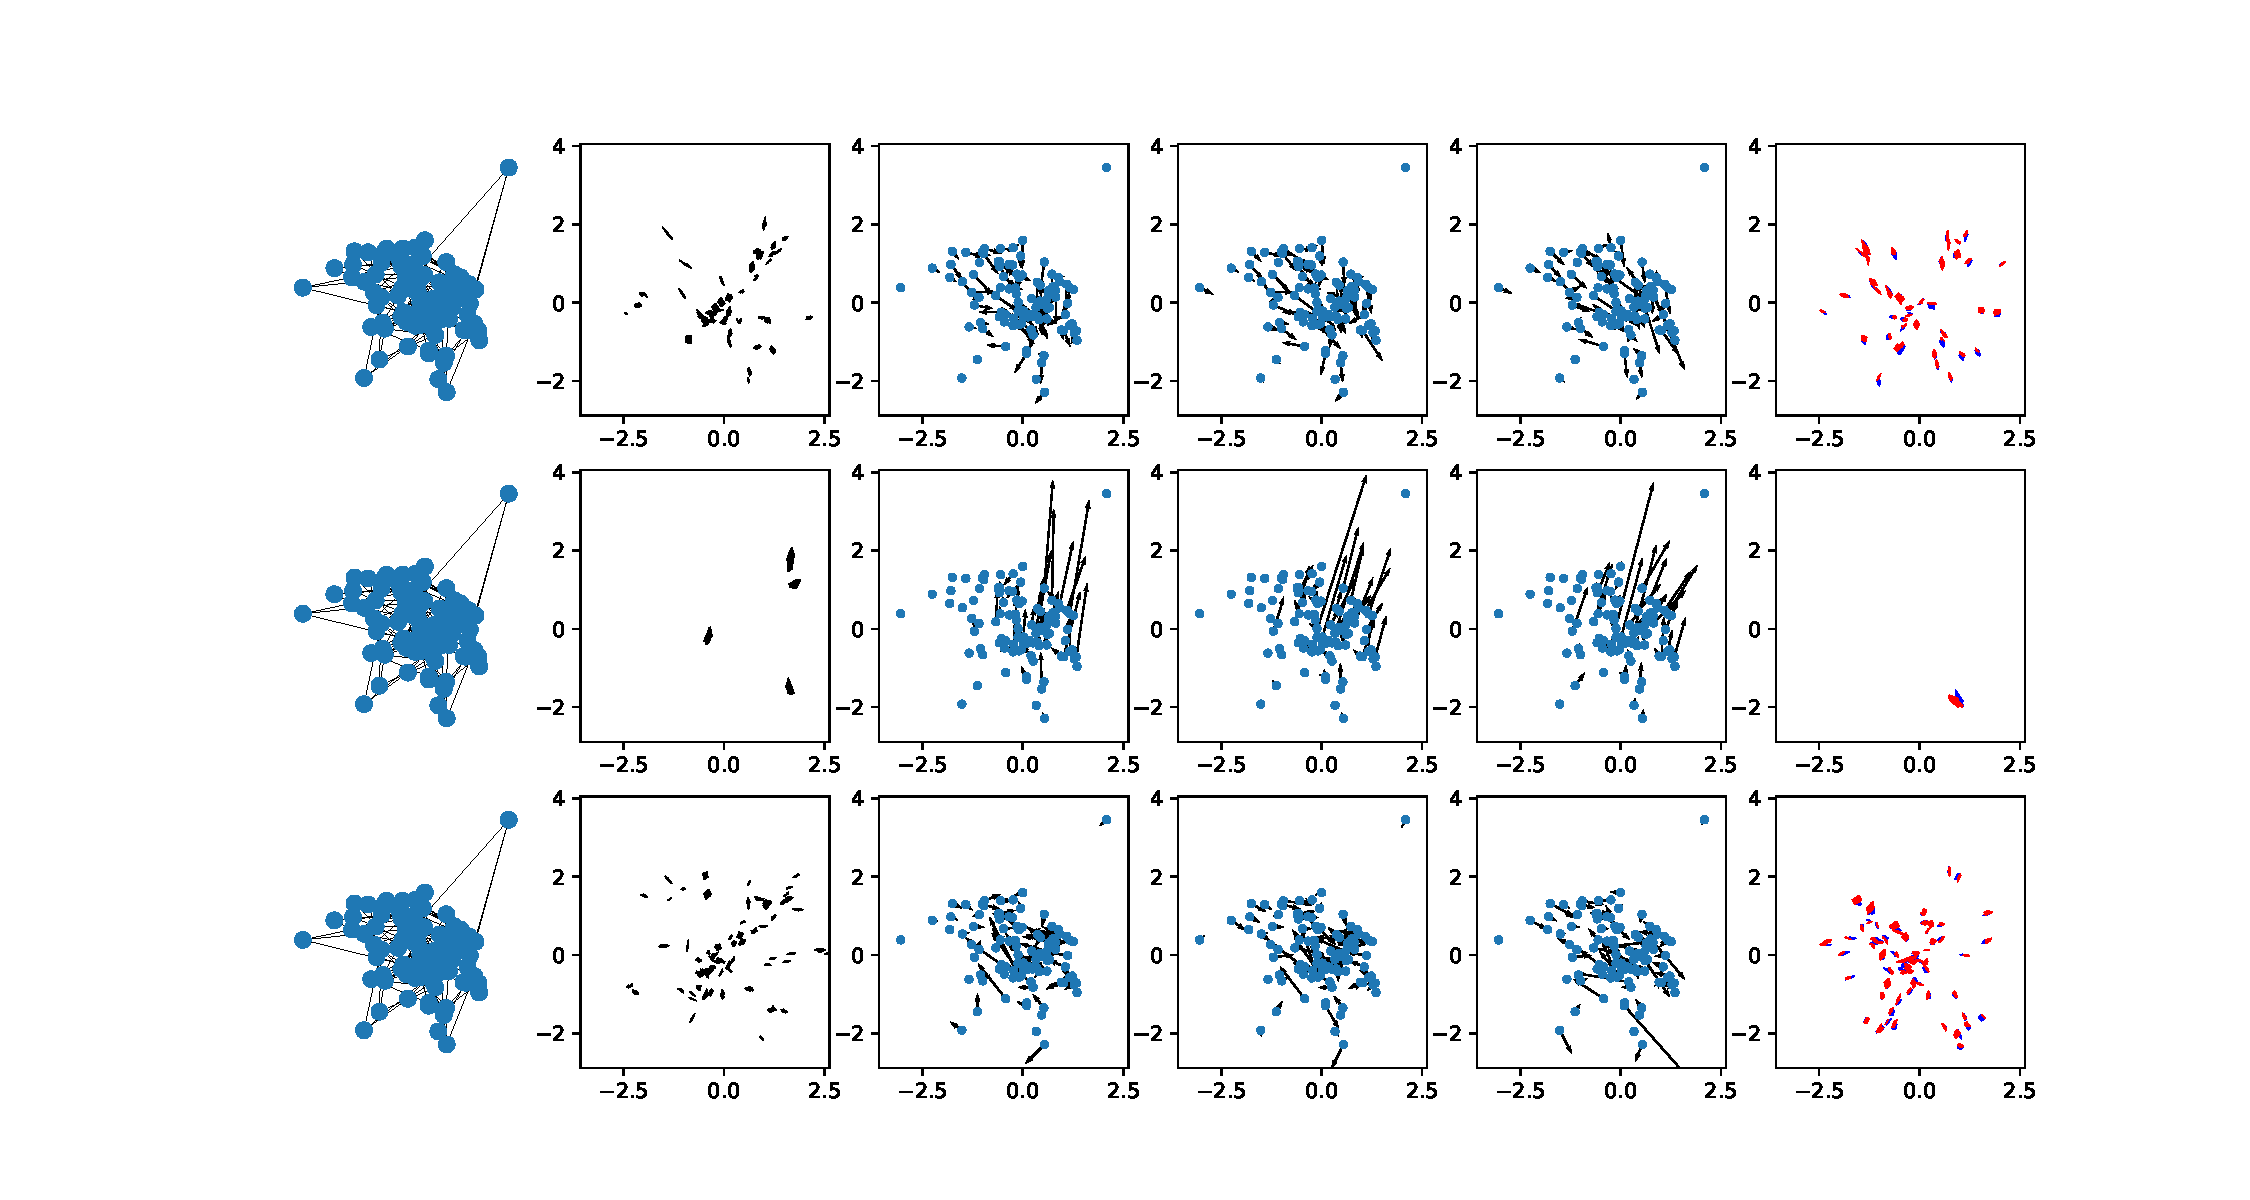
\includegraphics[trim={4.8cm 13.2cm 29.3cm 2.4cm},clip,width=0.7\textwidth]{../results/pdfs/nn-100N-noemb0}
            \caption{$k$-means, 3nn}
        \end{subfigure}
        \begin{subfigure}{0.24\textwidth}
            \centering
            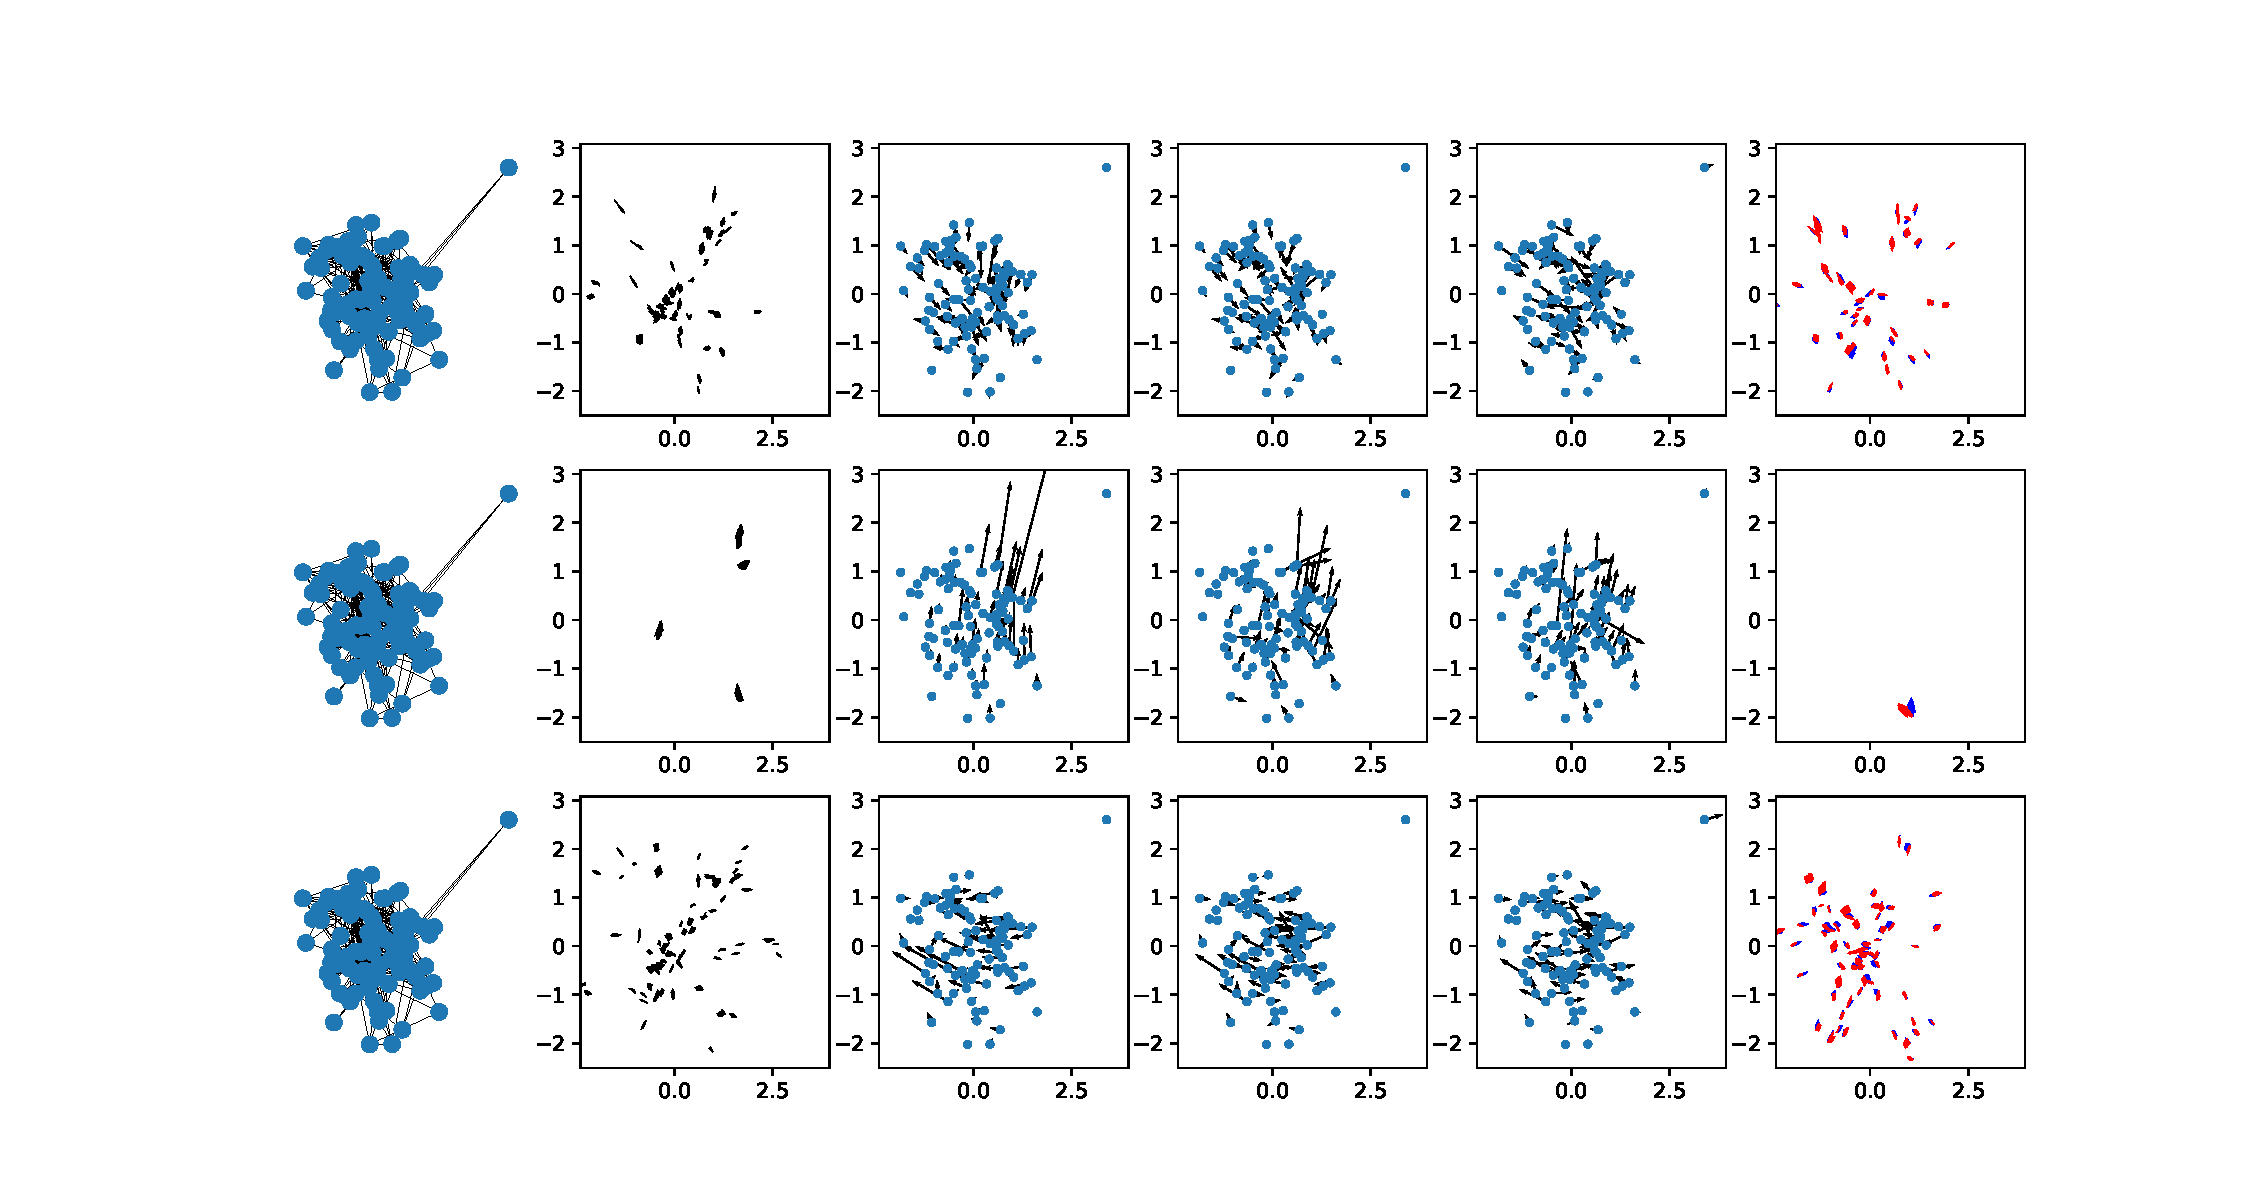
\includegraphics[trim={4.8cm 13.2cm 29.3cm 2.4cm},clip,width=0.7\textwidth]{../results/pdfs/ba-100N-noemb0}
            \caption{$k$-means, BA}
        \end{subfigure}
    \end{figure}
\end{frame}

\begin{frame}{Graph Types}
    \centering
    \begin{tabular}{lcccc} \toprule
        \multirow{2}{*}{\textbf{Model}}                      &                            & \multicolumn{3}{c}{\textbf{Nodes}}                                                           \\ \cmidrule(lr){3-5}
                                                             &                            & 10                                 & 100                    & 1000                           \\ \hline
        \multirow{2}{*}{\textbf{Random Network, $p=1\%$} }   & \scriptsize \textsc{Fixed} & 0.80  \tiny $\pm$ 0.04             & 0.71  \tiny $\pm$ 0.02 & 0.70 \tiny $\pm$ 0.02          \\
                                                             & \scriptsize \textsc{Adapt} & 0.69 \tiny $\pm$ 0.01              & 0.65 \tiny $\pm$ 0.02  & \textbf{0.64 \tiny $\pm$ 0.02} \\
        \multirow{2}{*}{\textbf{Random Network, $p=10\%$}}   & \scriptsize \textsc{Fixed} & 0.76  \tiny $\pm$ 0.03             & 0.70  \tiny $\pm$ 0.02 & 0.76 \tiny $\pm$ 0.02          \\
                                                             & \scriptsize \textsc{Adapt} & 0.69 \tiny $\pm$ 0.01              & 0.66 \tiny $\pm$ 0.01  & 0.66 \tiny $\pm$ 0.02          \\
        \multirow{2}{*}{\textbf{$k$-means, 3 nn.}          } & \scriptsize \textsc{Fixed} & 0.68  \tiny $\pm$ 0.01             & 0.69  \tiny $\pm$ 0.02 & 0.68 \tiny $\pm$ 0.01          \\
                                                             & \scriptsize \textsc{Adapt} & 0.68 \tiny $\pm$ 0.01              & 0.66 \tiny $\pm$ 0.01  & 0.65 \tiny $\pm$ 0.01          \\
        \multirow{2}{*}{\textbf{$k$-means, BA}             } & \scriptsize \textsc{Fixed} & 0.69  \tiny $\pm$ 0.01             & 0.68  \tiny $\pm$ 0.01 & 0.66 \tiny $\pm$ 0.02          \\
                                                             & \scriptsize \textsc{Adapt} & 0.68 \tiny $\pm$ 0.02              & 0.65 \tiny $\pm$ 0.02  & \textbf{0.64 \tiny $\pm$ 0.01} \\

        \bottomrule
    \end{tabular}
\end{frame}
\begin{frame}{Positional Encodings}
    \begin{figure}
        \begin{subfigure}{0.4\textwidth}
            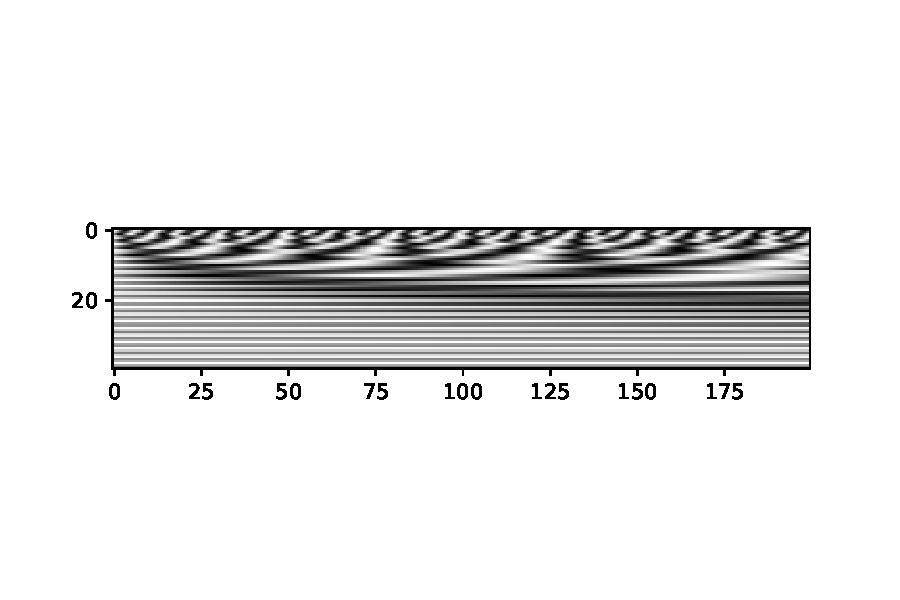
\includegraphics[width=\textwidth]{../windgraph/1dposenc}
        \end{subfigure}
        \begin{subfigure}{0.5\textwidth}
            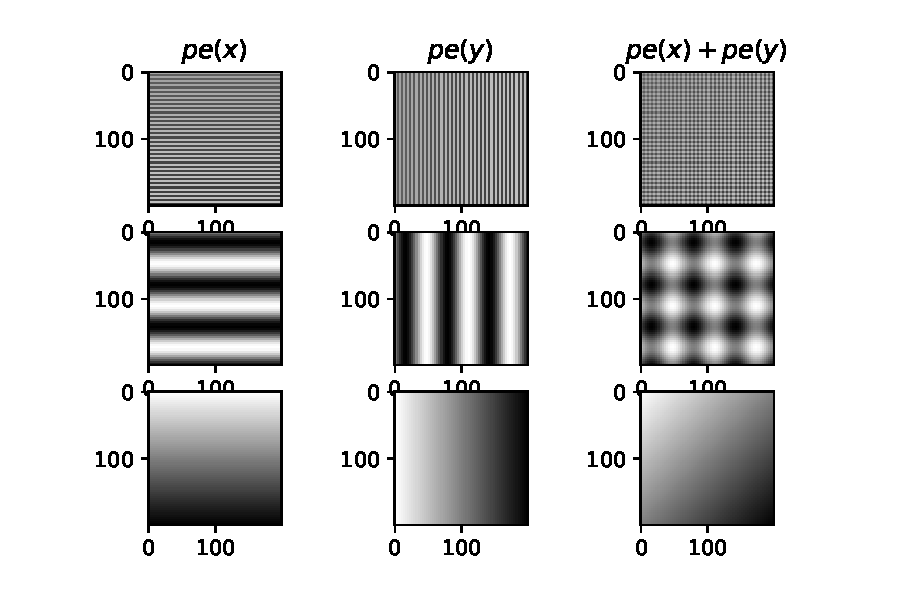
\includegraphics[width=\textwidth]{../windgraph/posenc}
        \end{subfigure}
    \end{figure}
\end{frame}

\begin{frame}
    \centering
    \begin{tabular}{lcccc} \toprule
        \multirow{2}{*}{\textbf{Model}}              &                            & \multicolumn{3}{c}{\textbf{Nodes}}                                                          \\ \cmidrule(lr){3-5}
                                                     &                            & 10                                 & 100                            & 1000                  \\ \hline
        \multirow{2}{*}{\textbf{No Emb}}             & \scriptsize \textsc{Fixed} & 0.68 \tiny $\pm$ 0.01              & 0.69 \tiny $\pm$ 0.02          & 0.68 \tiny $\pm$ 0.01 \\
                                                     & \scriptsize \textsc{Adapt} & 0.68 \tiny $\pm$ 0.01              & 0.66 \tiny $\pm$ 0.01          & 0.65 \tiny $\pm$ 0.01 \\
        \multirow{2}{*}{\textbf{MLP}}                & \scriptsize \textsc{Fixed} & 0.66 \tiny $\pm$ 0.01              & 0.66 \tiny $\pm$ 0.02          & 0.67 \tiny $\pm$ 0.02 \\
                                                     & \scriptsize \textsc{Adapt} & 0.66 \tiny $\pm$ 0.01              & 0.64 \tiny $\pm$ 0.01          & 0.64 \tiny $\pm$ 0.03 \\
        \multirow{2}{*}{\textbf{Added Pos-Enc,MLP}}  & \scriptsize \textsc{Fixed} & 1.03 \tiny $\pm$ 0.04              & 1.06 \tiny $\pm$ 0.02          & 1.04 \tiny $\pm$ 0.02 \\
                                                     & \scriptsize \textsc{Adapt} & 1.07 \tiny $\pm$ 0.07              & 1.04 \tiny $\pm$ 0.03          & 1.03 \tiny $\pm$ 0.02 \\
        \multirow{2}{*}{\textbf{Concat Pos-Enc,MLP}} & \scriptsize \textsc{Fixed} & 0.65 \tiny $\pm$ 0.01              & 0.63 \tiny $\pm$ 0.01          & 0.65 \tiny $\pm$ 0.02 \\
                                                     & \scriptsize \textsc{Adapt} & 0.65 \tiny $\pm$ 0.02              & \textbf{0.63 \tiny $\pm$ 0.01} & 0.64 \tiny $\pm$ 0.01 \\
        \bottomrule
    \end{tabular}
\end{frame}

\begin{frame}
    \begin{figure}[htbp]
        \centering
        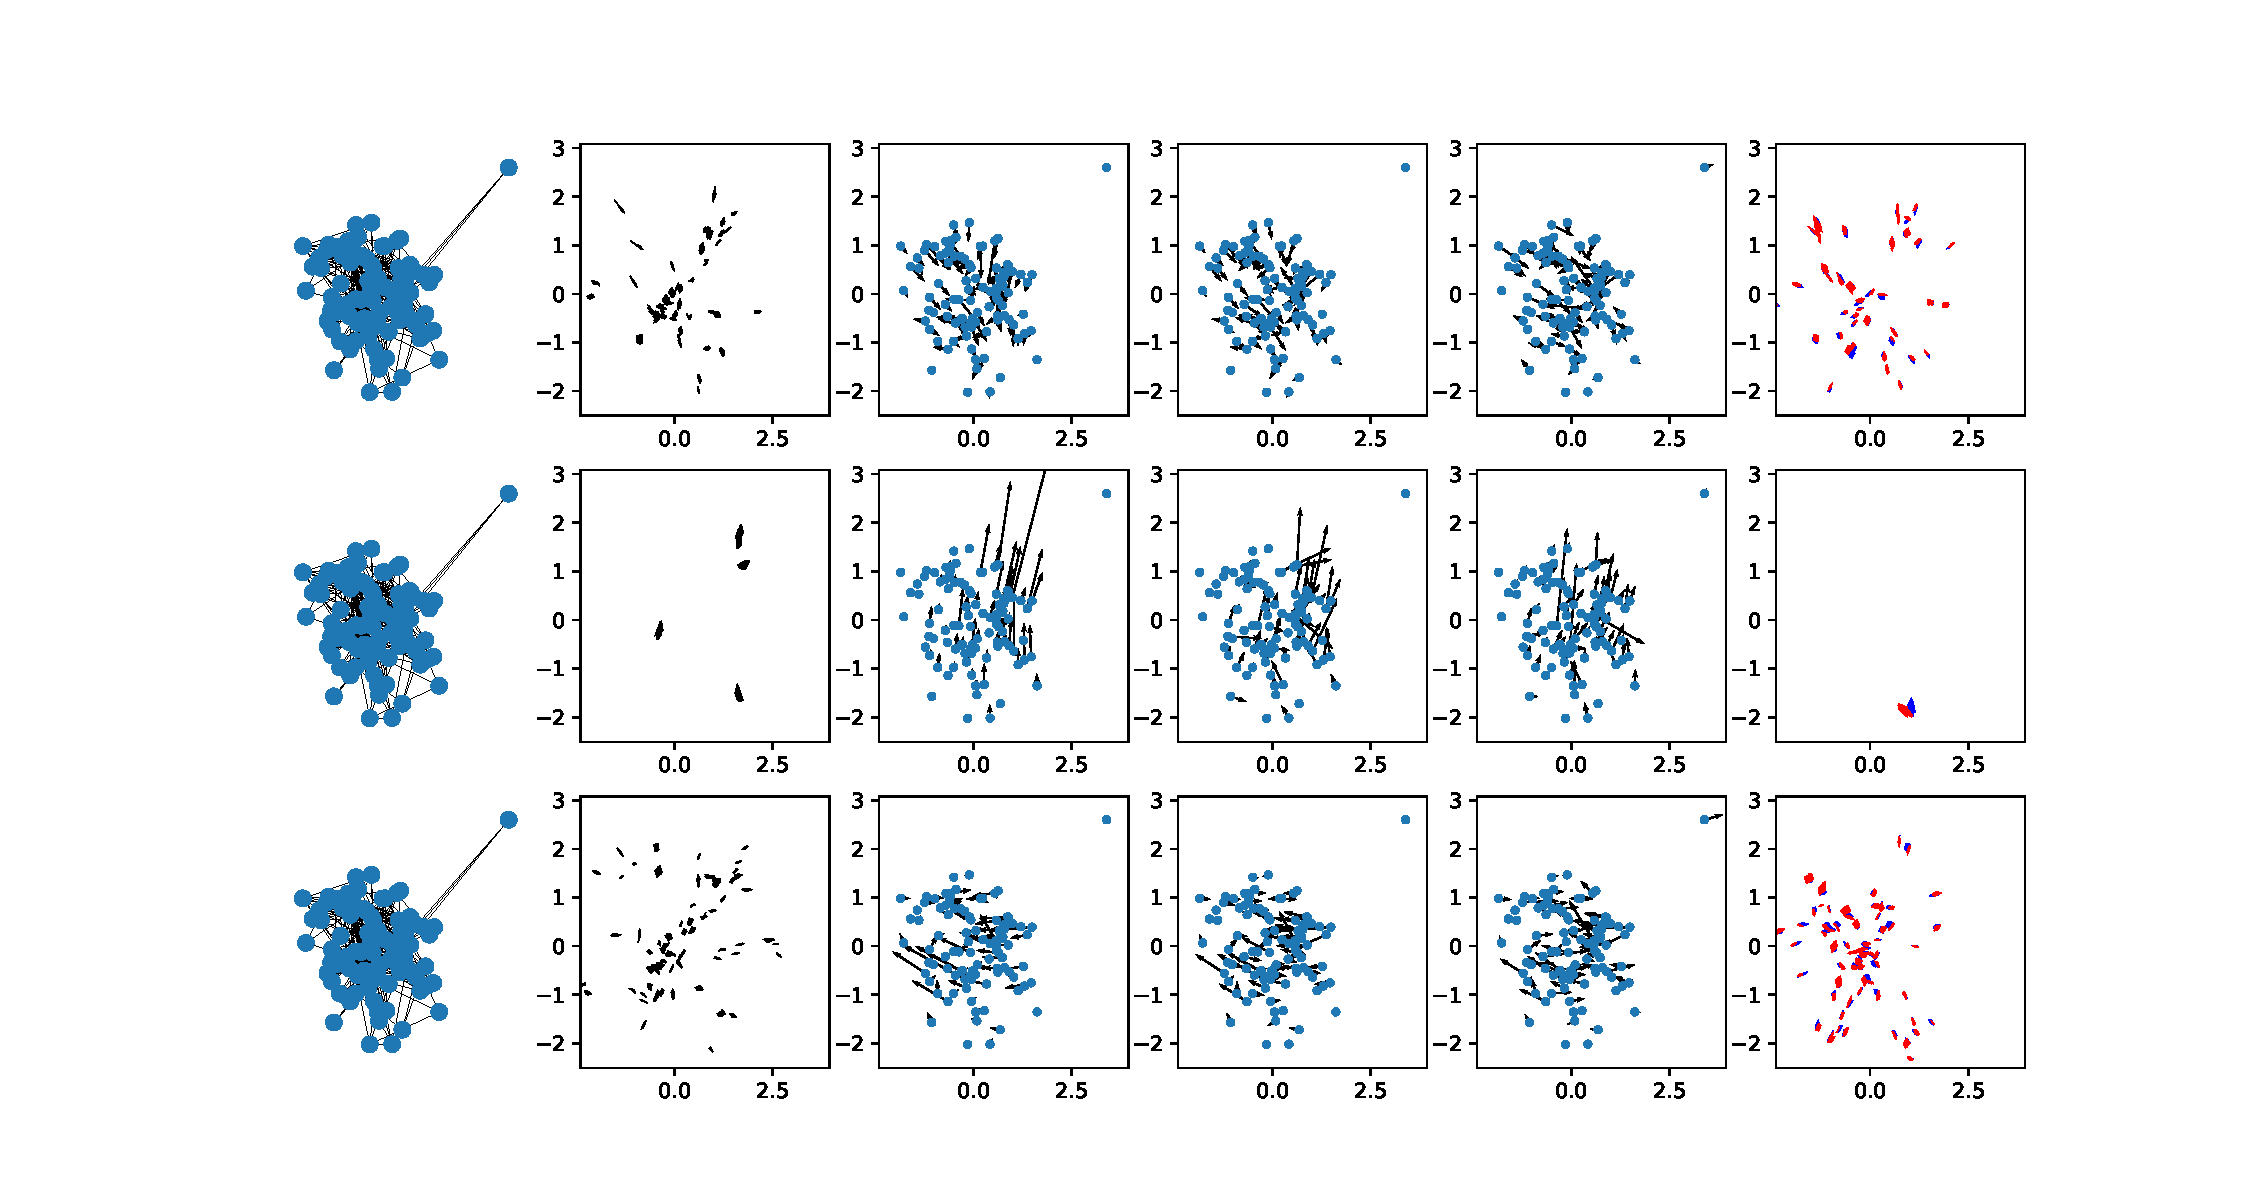
\includegraphics[width=\textwidth]{../results/pdfs/ba-100N-noemb0.pdf}
    \end{figure}
\end{frame}

\begin{frame}{Edge Features}
    \centering
    Idea : Encoding some values to help learning
    \begin{align*}
        \frac{u_{i}^{n + 1} - u_i^{n}}{\Delta t} = F_{i}^{n}(u,x,t, \frac{\partial u}{\partial x}, i\frac{\partial^2 u}{\partial x^{2}}    )
    \end{align*}
\end{frame}

\begin{frame}{Edge Features}
    \centering
    \begin{tabular}{lcccc} \toprule
        \multirow{2}{*}{\textbf{Edge Features}} &                            & \multicolumn{3}{c}{\textbf{Nodes}}                                                          \\ \cmidrule(lr){3-5}
                                                &                            & 10                                 & 100                   & 1000                           \\ \hline
        \textbf{Encoded distance}               & \scriptsize \textsc{Adapt} & 0.64 \tiny $\pm$ 0.02              & 0.63 \tiny $\pm$ 0.01 & 0.63 \tiny $\pm$ 0.01          \\
        \textbf{Encoded Finite difference}      & \scriptsize \textsc{Adapt} & 0.64 \tiny $\pm$ 0.02              & 0.63 \tiny $\pm$ 0.01 & \textbf{0.62 \tiny $\pm$ 0.01} \\ \hline
        \bottomrule
    \end{tabular}
\end{frame}

\begin{frame}
    \begin{columns}
        \begin{column}{0.4\textwidth}
            \coltitle{Conclusion} \\
            \vspace{10pt}
            Our best graph network uses:
            \begin{itemize}
                \item Long-range connection and hubs
                \item Positional Encodings
                \item Edge features encoding finite differences
            \end{itemize}

        \end{column}
        \begin{column}{0.6\textwidth}
            \centering
            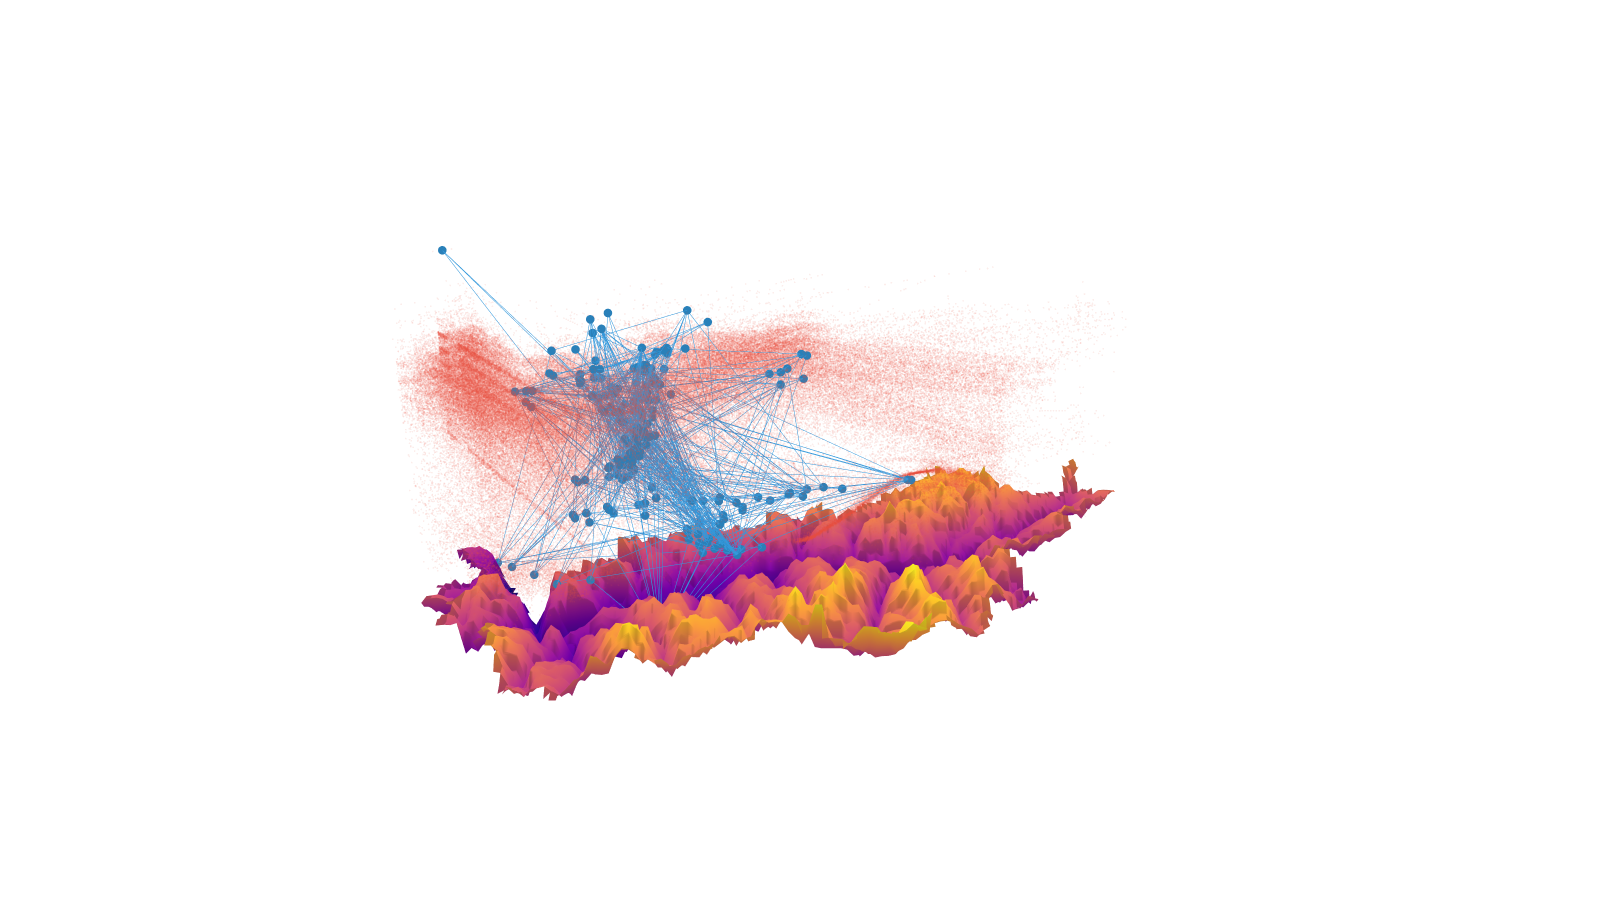
\includegraphics[trim={13cm 6cm 15cm 8cm},clip,width=\textwidth]{imgs/south-gen.png}
        \end{column}
    \end{columns}
\end{frame}


\begin{colorframe}
    \begin{frame}[plain]{Bibliography}
        \bibliography{slides}
        \bibliographystyle{apalike}
    \end{frame}
\end{colorframe}

\begin{frame}{Model Comparison}
    \centering
    \begin{tabular}{lc} \toprule
        \textbf{Model}                               & Norm. MSE     \\ \hline
        CNP \cite{garnelo2018conditional}            & 1.17          \\
        GKA - MLP \cite{pannatier2022windnowcasting} & 0.71          \\
        \textbf{Best GN}                             & \textbf{0.62} \\
        \textbf{Transformer}                         & \textbf{0.62} \\
        \bottomrule
    \end{tabular}
\end{frame}


\end{document}